\باب{پوئسن اور لاپلاس مساوات}
گاوس کے قانون کی نقطہ شکل
\begin{align}
\nabla \cdot \kvec{D}=\rho_h
\end{align}
میں \عددیء{\kvec{D}=\epsilon \kvec{E}} اور حاصل جواب میں \عددیء{\kvec{E}=-\nabla V} پر کرنے سے
\begin{align*}
\nabla \cdot (\epsilon \kvec{E})=-\nabla \cdot (\epsilon \nabla V)=\rho_h 
\end{align*}
یعنی
\begin{align}\label{مساوات_پوئسن_نقطہ}
\nabla \cdot \nabla V=-\frac{\rho_h}{\epsilon}
\end{align}
حاصل ہوتا ہے  جہاں ہر طرف یکساں\فرہنگ{یکساں!ہر طرف}\حاشیہب{homogeneous}\فرہنگ{homogeneous} خاصیت کے خطے میں \عددیء{\epsilon} اٹل قیمت رکھتا ہے۔مساوات \حوالہ{مساوات_پوئسن_نقطہ} \اصطلاح{پوئسن}\فرہنگ{پوئسن مساوات}\حاشیہب{Poisson equation}\فرہنگ{Poisson equation} مساوات  کہلاتی ہے۔

آئیں کارتیسی محدد میں پوئسن مساوات کی شکل حاصل کریں۔یاد رہے کہ کسی بھی متغیرہ \عددیء{\kvec{A}=A_x\ax+A_y\ay+A_z\az} کے لئے
\begin{align*}
\nabla \cdot \kvec{A}=\frac{\partial A_x}{\partial x}+\frac{\partial A_y}{\partial y}+\frac{\partial A_z}{\partial z}
\end{align*}  
کے برابر ہوتا ہے۔اب چونکہ
\begin{align*}
\nabla{V}=\frac{\partial V}{\partial x}\ax+\frac{\partial V}{\partial y}\ay+\frac{\partial V}{\partial z}\az
\end{align*}
 کے برابر ہے لہٰذا
\begin{gather}
\begin{aligned}
\nabla \cdot \nabla V&=\frac{\partial }{\partial x}\left(\frac{\partial V}{\partial x}\right)+\frac{\partial }{\partial y}\left(\frac{\partial V}{\partial y}\right)+\frac{\partial }{\partial z}\left(\frac{\partial V}{\partial z}\right)\\
&=\frac{\partial^2 V}{\partial x^2}+\frac{\partial^2 V}{\partial y^2}+\frac{\partial^2 V}{\partial z^2}
\end{aligned}
\end{gather}
 ہو گا۔

عموماً \عددیء{\nabla \cdot \nabla} کو \عددیء{\nabla^2} لکھا جاتا ہے۔اس طرح پوئسن مساوات کی کارتیسی شکل
\begin{align}\label{مساوات_لاپلاس_پوئسن_کارتیسی_شکل}
\nabla^2 V=\frac{\partial^2 V}{\partial x^2}+\frac{\partial^2 V}{\partial y^2}+\frac{\partial^2 V}{\partial z^2}=-\frac{\rho_h}{\epsilon}
\end{align}
حاصل ہوتی ہے۔ 

حجمی کثافتِ بار کی غیر موجودگی، یعنی \عددیء{\rho_h =0} کی صورت میں مساوات \حوالہ{مساوات_پوئسن_نقطہ}
\begin{align}\label{مساوات_لاپلاس_لاپلاس_نقطہ_شکل}
\nabla^2 V=0
\end{align}
صورت اختیار کر لے گی جسے \اصطلاح{لاپلاس}\فرہنگ{لاپلاس مساوات}\حاشیہب{Laplace equation}\فرہنگ{Laplace equation} مساوات کہتے ہیں۔جس حجم کے لئے لاپلاس کی مساوات لکھی گئی ہو اس حجم میں حجمی کثافتِ بار صفر ہوتا ہے البتہ اس حجم کی سرحد پر نقطہ بار یا سطحی کثافتِ بار پائی جا سکتیں ہیں۔عموماً سطح پر موجود بار سے حجم میں پیدا میدان ہی حاصل کرنا مطلوب ہوتا ہے۔کارتیسی محدد میں لاپلاس کی مساوات
\begin{align}\label{مساوات_لاپلاس_لاپلاس_کارتیسی_شکل}
\nabla^2 V=\frac{\partial^2 V}{\partial x^2}+\frac{\partial^2 V}{\partial y^2}+\frac{\partial^2 V}{\partial z^2}=0
\end{align}
صورت رکھتی ہے۔\عددیء{\nabla^2} کو لاپلاسی عامل\فرہنگ{لاپلاسی عامل}\حاشیہب{Laplacian operator}\فرہنگ{Laplacian operator} کہا جاتا ہے۔

لاپلاس مساوات کہتی ہے کہ کسی بھی بار سے خالی حجم میں ہر صورت \عددیء{\nabla^2V=0} ہو گا۔حجم کی شکل کچھ بھی ہو سکتی ہے اور اس کی سرحد پر کسی بھی قسم کا بار ہو سکتا ہے۔یہ ایک دلچسپ حقیقت ہے۔حجم کی سرحد پر عموماً ایک یا ایک سے زیادہ موصل سطحیں ہوتی ہیں جن پر برقی دباو \عددیء{V_0}، \عددیء{V_1}، \عددیء{V_2} وغیرہ پایا جاتا ہے اور حجم کے اندر میدان کا حصول درکار ہوتا ہے۔کبھی کبھار موصل سطح پر بار یا \عددیء{\kvec{E}} معلوم ہو گا جس سے حجم کے اندر میدان درکار ہو گا۔اسی طرح کبھی کبھار سرحد پر ایک جگہ بار اور اس پر دوسری جگہ برقی دباو اور اس پر تیسری  جگہ عمودی بہاو دیا گیا ہو گا جبکہ حجم کے اندر کے متغیرات درکار ہوں گے۔اس کے برعکس ایسا بھی ممکن ہے کہ حجم میں میدان یا برقی دباو معلوم ہو اور ان معلومات سے سرحد پر بار یا بہاو یا برقی دباو حاصل کرنا ضروری ہو گا۔

یہاں یہ بتلانا ضروری ہے کہ \عددیء{V=0} لاپلاس مساوات کا حل ہے۔یہ حل برقی دباو کی عدم موجودگی کو ظاہر کرتا ہے۔ہمیں عموماً ایسے مسئلوں سے دلچسپی ہوتی ہے جہاں برقی دباو پایا جائے۔اس لئے  لاپلاس مساوات کے اس حل کو ہم عموماً نظرانداز کریں گے۔ 

ہم نے لاپلاس کی مساوات برقی دباو کے لئے حاصل کی۔دیکھا یہ گیا ہے کہ انجینئری کے دیگر شعبوں میں کئی متغیرات لاپلاس کی مساوات پر پورا اترتے ہیں۔یہ مساوات حقیقی اہمیت کا حامل ہے۔ 

اس باب میں ہم ایسی کئی مثالیں دیکھیں گے لیکن پہلے یہ حقیقت جاننا ضروری ہے کہ مساوات \حوالہ{مساوات_لاپلاس_لاپلاس_کارتیسی_شکل} کا کوئی بھی جواب ان تمام اقسام کی سرحدی معلومات کے لئے درست ہو گا۔یہ انتہائی تشویشناک بات ہو گی اگر دو مختلف طریقوں سے لاپلاس مساوات کے جوابات حاصل کرنے کے بعد معلوم ہو کہ ان میں سے ایک ٹھیک اور دوسرا غلط جواب ہے۔آئیں اس حقیقت کا ثبوت دیکھیں کہ کسی بھی سرحدی حقائق کو مد نظر رکھتے ہوئے لاپلاس مساوات کا صرف اور صرف ایک ہی جواب حاصل ہوتا ہے۔
%===================================

\ابتدا{مثال}
لاپلاس اور پوئسن  کی مساوات حاصل کرتے وقت پورے خطے میں یکساں \عددی{\epsilon} تصور کی گئی۔غیر یکساں \عددی{\epsilon} کی صورت میں \عددی{\epsilon} کی تبدیلی پر وہ شرط حاصل کریں جس سے لاپلاس اور پوئسن مساوات برقرار رہتے ہیں۔

حل: مساوات \عددی{\nabla \cdot \kvec{D}=\rho_h} سے شروع کرتے ہیں جس میں \عددی{\kvec{D}=\epsilon \kvec{E}} پر کرتے ہوئے آگے بڑھتے ہیں۔ سمتی \عددی{\kvec{E}} اور غیر سمتی \عددی{\epsilon} کی صورت میں
\begin{align*}
\nabla \cdot \kvec{D}=\nabla \cdot (\epsilon \kvec{E})=\kvec{E} \cdot \nabla \epsilon+\epsilon \nabla \cdot \kvec{E}=\rho_h
\end{align*}
لکھا جا سکتا ہے۔  اس میں \عددی{\kvec{E}=-\nabla V} پر کرنے سے
\begin{align*}
-\nabla V \cdot \nabla \epsilon-\epsilon \nabla^2 V=\rho_h
\end{align*}
حاصل ہوتا ہے۔اس مساوات سے پوئسن مساوات اس صورت حاصل ہو گی جب \عددی{\nabla V \cdot \nabla \epsilon=0} یعنی \عددی{\kvec{E} \cdot \nabla \epsilon=0} ہو۔ایسا ہونے کا مطلب ہے  کہ کسی بھی نقطے پر  \عددی{\epsilon} میں تبدیلی کی سمت، اسی نقطے پر \عددی{\kvec{E}} کے سمت کے عمودی ہو۔ 
\انتہا{مثال}

%===================================
\حصہ{مسئلہ یکتائی}
تصور کریں کہ ہم دو مختلف طریقوں سے لاپلاس مساوات کے دو جوابات \عددیء{V_1} اور \عددیء{V_2} حاصل کرتے ہیں۔یہ دونوں جوابات لاپلاس مساوات پر پورا اترتے ہیں لہٰذا
\begin{align*}
\nabla^2 V_1&=0\\
\nabla^2 V_2&=0
\end{align*} 
لکھا جا سکتا ہے جس سے
\begin{align}\label{مساوات_لاپلاس_دو_جوابات_الف}
\nabla^2 (V_1-V_2)=0
\end{align}
حاصل ہوتا ہے۔اب اگر سرحد پر برقی دباو \عددیء{V_s} ہو تب دونوں جوابات سرحد پر یہی جواب دیں گے یعنی سرحد پر
\begin{align*}
V_{1s}=V_{2s}=V_s
\end{align*}
یا
\begin{align*}
V_{1s}-V_{2s}=0
\end{align*}
ہو گا۔صفحہ \حوالہصفحہ{مساوات_توانائی_توانائی_ضرب_برقی_بہاو_کی_ڈھلوان} پر مساوات \حوالہ{مساوات_توانائی_توانائی_ضرب_برقی_بہاو_کی_ڈھلوان}
\begin{align*}
\nabla \cdot  (V \kvec{D})=V (\nabla \cdot \kvec{D})+\kvec{D} \cdot (\nabla V)
\end{align*}
کا ذکر کیا گیا جو کسی بھی غیر سمتی مقدار \عددیء{V} اور کسی بھی سمتیہ \عددیء{\kvec{D}} کے لئے درست ہے۔موجودہ استعمال کے لئے ہم \عددیء{V_1-V_2} کو غیر سمتی اور \عددیء{\nabla(V_1-V_2)} کو سمتیہ لیتے ہوئے
\begin{align*}
\nabla \cdot  [(V_1-V_2) \nabla(V_1-V_2)]&=(V_1-V_2) [\nabla \cdot \nabla(V_1-V_2)]+\nabla(V_1-V_2) \cdot \nabla (V_1-V_2)\\
&=(V_1-V_2) [\nabla^2(V_1-V_2)]+[\nabla(V_1-V_2)]^2
\end{align*}
لکھ سکتے ہیں جس کا تکمل پورے حجم کے لئے
\begin{equation}\label{مساوات_لاپلاس_یکتائی_ثبوت_الف}
\resizebox{.9\hsize}{!}{$
\int\limits_{\text{حجم}} \nabla \cdot  [(V_1-V_2) \nabla(V_1-V_2)] \dif h=\int\limits_{\text{حجم}}(V_1-V_2) [\nabla^2(V_1-V_2)] \dif h+\int\limits_{\text{حجم}}[\nabla(V_1-V_2)]^2 \dif h $}
\end{equation}
ہو گا۔صفحہ \حوالہصفحہ{مساوات_گاوس_مسئلہ_پھیلاو_تکمل_شکل} پر مساوات \حوالہ{مساوات_گاوس_مسئلہ_پھیلاو_تکمل_شکل} مسئلہ پھیلاو بیان کرتا ہے جس کے مطابق کسی بھی حجمی تکمل کو  بند سطحی تکمل میں تبدیل کیا جا سکتا ہے جہاں حجم کی سطح پر سطحی تکمل حاصل کیا جاتا ہے۔یوں مندرجہ بالا مساوات کے بائیں ہاتھ کو سطحی تکمل میں تبدیل کرتے ہوئے
\begin{align*}
\int\limits_{\text{حجم}} \nabla \cdot  [(V_1-V_2) \nabla(V_1-V_2)] \dif h=\oint\limits_{\text{سطح}} [(V_{1s}-V_{2s}) \nabla(V_{1s}-V_{2s})] \cdot \dif \kvec{S}=0
\end{align*}
حاصل ہوتا ہے جہاں سرحدی سطح پر \عددیء{V_{1s}=V_{2s}} ہونے کی بنا پر \عددیء{V_{1s}-V_{2s}=0} ہے اور صفر کا تکمل صفر ہی ہوتا ہے۔مساوات \حوالہ{مساوات_لاپلاس_یکتائی_ثبوت_الف} میں دائیں ہاتھ پہلے جزو میں مساوات \حوالہ{مساوات_لاپلاس_دو_جوابات_الف} کے تحت \عددیء{\nabla^2(V_1-V_2)=0} ہے اور صفر کا تکمل صفر ہی ہوتا ہے۔اس طرح مساوات \حوالہ{مساوات_لاپلاس_یکتائی_ثبوت_الف} سے
\begin{align*}
\int\limits_{\text{حجم}}[\nabla(V_1-V_2)]^2 \dif h=0
\end{align*}
حاصل ہوتی ہے۔

کسی بھی تکمل کا جواب صرف دو صورتوں میں صفر کے برابر ہو سکتا ہے۔پہلی صورت یہ ہے کہ کچھ خطے میں تکمل کی قیمت مثبت اور کچھ خطے میں اس کی قیمت منفی ہو۔اگر مثبت اور منفی حصے بالکل برابر ہوں تب تکمل صفر کے برابر ہو گا۔موجودہ صورت میں \عددیء{[\nabla(V_1-V_2)]^2} کا تکمل لیا جا رہے ہے اور کسی بھی متغیر کا مربع کسی صورت منفی نہیں ہو سکتا لہٰذا موجودہ تکمل میں ایسا ممکن نہیں ہے۔تکمل صفر ہونے کی دوسری صورت یہ ہے کہ صفر کا تکمل حاصل کیا جا رہا ہو لہٰذا
\begin{align*}
[\nabla(V_1-V_2)]^2 =0
\end{align*}
ہی ہو گا یعنی
\begin{align*}
\nabla (V_1-V_2)=0
\end{align*}
کے برابر ہے۔

اب \عددیء{\nabla (V_1-V_2)=0} کا مطلب ہے کہ \عددیء{V_1-V_2} کی ڈھلوان ہر صورت صفر کے برابر ہے۔یہ تب ہی ممکن ہے جب \عددیء{V_1-V_2} کی قیمت کسی بھی محدد کے ساتھ تبدیل نہ ہو یعنی اگر تکمل کے پورے خطے میں
\begin{align*}
V_1-V_2=\text{اٹل قیمت}
\end{align*}
ہو۔حجم کی سرحد پر بھی یہ درست ہو گا۔مگر سرحد پر
\begin{align*}
V_1-V_2=V_{1s}-V_{2s}=0
\end{align*}
کے برابر ہے لہٰذا یہ اٹل قیمت ازخود صفر ہے۔یوں
\begin{align}
V_1=V_2
\end{align}
ہو گا۔اس کا مطلب  ہے کہ دونوں جوابات بالکل برابر ہیں۔

مسئلہ یکتائی کو پوئسن مساوات کے لئے بھی بالکل اسی طرح ثابت کیا جا سکتا ہے۔پوئسن مساوات کے دو جوابات \عددیء{V_1} اور \عددیء{V_2} پوئسن مساوات پر پورا اتریں گے لہٰذا \عددیء{\nabla^2 V_1=-\tfrac{\rho_h}{\epsilon}} اور \عددیء{\nabla^2 V_2=-\tfrac{\rho_h}{\epsilon}} لکھے جا سکتے ہیں جن سے \عددیء{\nabla^2(V_1-V_2)=0} حاصل ہوتا ہے۔سرحد پر اب بھی \عددیء{{V_{1s}-V_{2s}= 0}} ہو گا۔یہاں سے آگے ثبوت بالکل یکتائی لاپلاس کی ثبوت کی طرح ہے۔

مسئلہ یکتائی کے تحت سرحدی حقائق کے لئے حاصل کئے  گئے پوئسن یا لاپلاس مساوات کے جوابات ہر صورت برابر ہوں گے۔یہ ممکن نہیں کہ دو مختلف جوابات حاصل کئے جائیں۔ 

\حصہ{لاپلاس مساوات خطی ہے}
تصور کریں کہ سرحدی شرائط لاگو کرنے  کے بغیر لاپلاس مساوات کے دو حل \عددیء{V_1} اور \عددیء{V_2} حاصل کئے جائیں۔یوں
\begin{align*}
\nabla^2 V_1&=0\\
\nabla^2 V_2&=0
\end{align*}
لکھا جا سکتا ہے جن سے
\begin{align*}
\nabla^2 (c_1 V_1 + c_2 V_2)=0 
\end{align*}
بھی لکھا جا سکتا ہے جہاں \عددیء{c_1} اور \عددیء{c_2} مستقل ہیں۔اس حقیقت کو یوں بیان کیا جاتا ہے کہ لاپلاس مساوات \اصطلاح{خطی}\فرہنگ{خطی}\حاشیہب{linear}\فرہنگ{linear} ہے۔


\حصہ{نلکی اور کروی محدد میں لاپلاس کی مساوات} 
نلکی محدد میں ڈھلوان کی مساوات صفحہ \حوالہصفحہ{مساوات_توانائی_ڈھلوان_نلکی} پر مساوات \حوالہ{مساوات_توانائی_ڈھلوان_نلکی} دیتی ہے جس سے 
\begin{gather}
\begin{aligned}\label{مساوات_لاپلاس_نلکی_پھیلاو_الف}
\nabla V &= \frac{\partial V}{\partial \rho} \arho+\frac{1}{\rho}\frac{\partial V}{\partial \phi}  \aphi+\frac{\partial V}{\partial z}\az\\
&=-E_\rho \arho-E_\phi \aphi-E_z \az 
\end{aligned}
\end{gather}
لکھتے  ہیں جہاں \عددیء{\kvec{E}=-\nabla V} کا استعمال کیا گیا۔نلکی محدد میں پھیلاو کی مساوات صفحہ \حوالہصفحہ{مساوات_گاوس_نلکی_عمومی_پھیلاو} پر مساوات \حوالہ{مساوات_گاوس_نلکی_عمومی_پھیلاو} دیتا ہے۔اسی مساوات کو سمتیہ \عددیء{\kvec{E}} کے لئے
 \begin{align*}
\nabla \cdot \kvec{E}=\frac{1}{\rho}\frac{\partial (\rho E_{\rho})}{\partial \rho}+\frac{1}{\rho}\frac{\partial E_{\phi}}{\partial \phi}  +  \frac{\partial E_{z}}{\partial z}
\end{align*}
لکھتے ہیں۔اس میں بائیں ہاتھ \عددیء{\kvec{E}=-\nabla V}  اور دائیں ہاتھ مساوات \حوالہ{مساوات_لاپلاس_نلکی_پھیلاو_الف} سے قیمتیں پر کرتے ہوئے
\begin{align*}
\nabla \cdot \nabla V=\frac{1}{\rho}\frac{\partial }{\partial \rho}\left(\rho \frac{\partial V}{\partial \rho}\right)
+\frac{1}{\rho}\frac{\partial }{\partial \phi}\left(\frac{1}{\rho}\frac{\partial V}{\partial \phi}  \right) 
+  \frac{\partial}{\partial z} \left(\frac{\partial V}{\partial z} \right)
\end{align*}
حاصل ہوتا ہے جہاں دونوں جانب منفی علامت کٹ جاتے ہیں۔اس کو یوں
\begin{align}
\nabla^2 V=\frac{1}{\rho}\frac{\partial }{\partial \rho}\left(\rho \frac{\partial V}{\partial \rho}\right)
+\frac{1}{\rho^2}\left(\frac{\partial^2 V}{\partial \phi^2}  \right) 
+  \frac{\partial^2 V}{\partial z^2}\quad {\text{نلکی}}
\end{align}
 لکھا جا سکتا ہے جو نلکی محدد میں لاپلاسی مساوات ہے۔

کروی محدد میں بالکل اسی طرح
\begin{align}\label{مساوات_لاپلاس_کروی_لاپلاسی}
\nabla^2 V=\frac{1}{r^2} \frac{\partial}{\partial r} \left(r^2\frac{\partial V}{\partial r} \right)+\frac{1}{r^2 \sin \theta} \frac{\partial}{\partial \theta} \left(\sin \theta \frac{\partial V}{\partial \theta}  \right)+\frac{1}{r^2 \sin \theta}\frac{\partial^2 V}{\partial \phi^2} \quad {\text{کروی}}
\end{align}
جبکہ عمومی محدد میں
\begin{align}\label{مساوات_لاپلاس_عمومی_لاپلاسی}
\nabla^2 V=\frac{1}{k_1 k_2 k_3}\left[\frac{\partial}{\partial u}\left(\frac{k_2 k_3}{k_1}\frac{\partial V}{\partial u} \right)+\frac{\partial}{\partial v}\left(\frac{k_1 k_3}{k_2}\frac{\partial V}{\partial v} \right) +\frac{\partial}{\partial w}\left(\frac{k_1 k_2}{k_3}\frac{\partial V}{\partial w} \right)\right] \quad{\text{عمومی}}
\end{align}
حاصل کی جا سکتی ہے۔
%==================

\ابتدا{مشق}
مساوات \حوالہ{مساوات_لاپلاس_کروی_لاپلاسی} حاصل کریں۔
\انتہا{مشق}
%============================

\حصہ{لاپلاس مساوات کے حل}
لاپلاس مساوات حل کرنے کے کئی طریقے ہیں۔سادہ ترین مسئلے، سادہ تکمل سے ہی حل ہو جاتے ہیں۔ہم اسی سادہ تکمل کے طریقے سے کئی مسئلے حل کریں گے۔یہ طریقہ صرف اس صورت قابل استعمال ہوتا ہے جب میدان یک سمتی ہو یعنی جب یہ محدد کے تین سمتوں میں سے صرف ایک سمت میں تبدیل ہوتا ہو۔چونکہ اس کتاب میں محدد کے تین نظام استعمال کئے جا رہے ہیں لہٰذا معلوم ایسا ہوتا ہے کہ  کل نو مسئلے ممکن ہیں۔درحقیقت ایسا نہیں ہے۔کارتیسی محدد میں \عددیء{x} سمت میں تبدیل ہوتے میدان کا حل بالکل ویسا ہی ہے جیسے \عددیء{y} یا \عددیء{z} سمت میں تبدیل ہوتے میدان کا حل۔اسی طرح \عددیء{x} محدد سے کسی زاویے پر سیدھی لکیر کی سمت میں تبدیل ہوتا میدان بھی بالکل اسی طرح حل ہو گا۔یوں کارتیسی محدد میں کسی بھی سمت میں تبدیل ہوتے میدان اور \عددیء{x} سمت میں تبدیل ہوتے میدان کے حل بالکل ایک جیسے ہوں گے لہٰذا کارتیسی محدد میں صرف ایک مسئلہ حل کرنا درکار ہے۔نلکی محدد میں \عددیء{z} محدد کے ساتھ تبدیل ہوتے میدان کو ہم کارتیسی محدد میں دیکھ لیں گے لہٰذا یہاں کل دو مسئلے حل کرنا درکار ہے جبکہ کروی محدد میں بھی دو مسئلے پائے جاتے ہیں۔آئیں ان تمام کو باری باری حل کریں۔
%=================

\ابتدا{مثال}
تصور کریں کہ \عددیء{V} صرف \عددیء{x} محدد کے ساتھ تبدیل ہوتی ہو۔دیکھتے ہیں کہ ایسی صورت میں لاپلاس مساوات کا حل کیا ہو گا۔اس پر بعد میں غور کریں گے کہ حقیقت میں ایسی کون سی صورت ہو گی کہ \عددیء{V} صرف \عددیء{x} محدد کے ساتھ تبدیل ہوتا ہو۔ایسی صورت میں لاپلاس مساوات
\begin{align*}
\frac{\partial^2 V}{\partial x^2}=0
\end{align*}
شکل اختیار کر لے گا۔چونکہ \عددیء{V} کی قیمت صرف \عددیء{x} پر منحصر ہے لہٰذا مندرجہ بالا مساوات کو
\begin{align*}
\frac{\dif{\hspace{0.1pt} ^2} V}{\dif x^2}=0
\end{align*}
لکھا جا سکتا ہے۔پہلی مرتبہ تکمل لیتے ہوئے
\begin{align*}
\frac{\dif V}{\dif x}=A
\end{align*}
حاصل ہوتا ہے۔دوبارہ تکمل لیتے ہوئے
\begin{align}\label{مساوات_لاپلاس_کارتیسی_حل}
V=Ax+B
\end{align}
حاصل ہوتا ہے جو لاپلاس مساوات کا حل ہے۔یہ کسی بھی سیدھی لکیر کی سمت میں تبدیل ہوتے برقی دباو کے مسئلے کو ظاہر کرتا ہے جہاں اس لکیر کو \عددیء{x} کہا جائے گا۔\عددیء{A} اور \عددیء{B} دو درجی تکمل کے مستقل ہیں جن کی قیمتیں سرحدی شرائط کی مدد سے حاصل کی جاتی ہیں۔

آئیں مساوات \حوالہ{مساوات_لاپلاس_کارتیسی_حل} کا مطلب سمجھیں۔اس کے مطابق برقی دباو کا دارومدار صرف \عددیء{x} پر ہے  جبکہ \عددیء{y} اور \عددیء{z} کا اس کی قیمت پر کوئی اثر نہیں۔\عددیء{x} کی کسی بھی قیمت پر یعنی \عددیء{x=x_0} سطح پر \عددیء{V} کی قیمت اٹل ہو گی۔ایسی ہم قوہ سطحیں \عددیء{x} محدد کے عمودی ہوں گی۔آپ دیکھ سکتے ہیں کہ مساوات \حوالہ{مساوات_لاپلاس_کارتیسی_حل} یہ متوازی چادر برق گیر (کپیسٹر)  کا حل ہے۔

ہم ایسے برق گیر (کپیسٹر)  کے دونوں چادروں پر برقی دباو اور چادروں کا \عددیء{x} محدد پر مقام بیان کرتے ہوئے  \عددیء{A} اور \عددیء{B} کی قیمتیں حاصل کر سکتے ہیں۔یوں اگر برق گیر (کپیسٹر)  کی پہلی  چادر  \عددیء{x_1} پر ہے جبکہ اس پر برقی دباو \عددیء{V_1} ہے اور اسی طرح دوسری چادر \عددیء{x_2} پر ہے جبکہ اس پر برقی دباو \عددیء{V_2} ہے تب
\begin{align*}
V_1&=A x_1+B\\
V_2&=Ax_2+B
\end{align*}
ہو گا جس سے
\begin{align*}
A&=\frac{V_1-V_2}{x_1-x_2}\\
B&=\frac{V_2 x_1-V_1x_2}{x_1-x_2}
\end{align*}
حاصل ہوتے ہیں۔یوں چادروں کے درمیان
\begin{align}
V=\left(\frac{V_1-V_2}{x_1-x_2}\right)x+\frac{V_2 x_1-V_1x_2}{x_1-x_2}
\end{align}
ہو گا۔

اگر ہم پہلی  چادر کو \عددیء{x=0} اور دوسری چادر کو \عددیء{d} پر تصور کرتے جبکہ اسی ترتیب سے ان کی برقی دباو کو صفر اور \عددیء{V_0} کہتے تب ہمیں
\begin{align}\label{مساوات_لاپلاس_کارتیسی_برقی_دباو}
V=\frac{V_0 x}{d}
\end{align}
حاصل ہوتا جو نسبتاً آسان مساوات ہے۔

باب \حوالہ{باب_کپیسٹر} میں ہم نے سطحی کثافتِ بار سے بالترتیب برقی میدان، برقی دباو اور کپیسٹنس حاصل کئے۔موجودہ باب میں ہم پہلے لاپلاس کی مساوات کے حل سے برقی دباو حاصل کرتے ہیں۔برقی دباو سے میدان بذریعہ  \عددیء{\kvec{E}=-\nabla V} اور بہاو بذریعہ \عددیء{\kvec{D}=\epsilon \kvec{E}} حاصل کرتے ہوئے سطحی کثافتِ بار حاصل کرتے ہیں جو عمودی بہاو کے برابر ہے۔سطحی کثافتِ بار سے سطح پر کل بار حاصل کرتے ہوئے \عددیء{C=\tfrac{Q}{V}} حاصل کیا جاتا ہے۔ان اقدام کو بالترتیب دوبارہ پیش کرتے ہیں۔
\begin{itemize}
\item
لاپلاس مساوات حل کرتے ہوئے برقی دباو \عددیء{V} حاصل کریں۔
\item
تکمل کی سرحدی شرائط سے تکمل کے مستقل کی قیمتیں حاصل کریں۔
\item
برقی دباو سے برقی میدان اور برقی بہاو  بذریعہ \عددیء{\kvec{E}=-\nabla V} اور \عددیء{\kvec{D}=\epsilon \kvec{E}} حاصل کریں۔
\item
برق گیر (کپیسٹر)  کے کسی ایک چادر پر برقی بہاو کی قیمت \عددیء{\kvec{D}_S=D_n\aN} حاصل کریں جو سطح کے عمودی ہو گا۔ 
\item
چونکہ سطح پر سطحی کثافتِ بار اور عمودی برقی بہاو برابر ہوتے ہیں لہٰذا \عددیء{\rho_S=D_n} ہو گا۔مثبت کثافتِ بار کی صورت میں برقی بہاو کا موصل چادر سے اخراج جبکہ منفی کثافتِ بار کی صورت میں برقی بہاو کا چادر میں دخول ہو گا۔
\item
سطح پر بار بذریعہ سطحی تکمل حاصل کریں۔
\item
کپیسٹنس \عددیء{C=\tfrac{Q}{V}} ہو گا۔
\end{itemize}
آئیں ان اقدام کو موجودہ مثال پر لاگو کریں۔

چونکہ موجودہ مثال میں مساوات \حوالہ{مساوات_لاپلاس_کارتیسی_برقی_دباو} کے تحت
\begin{align*}
V=\frac{V_0x}{d}
\end{align*}
ہے لہٰذا
\begin{align*}
\kvec{E}=-\nabla V=-\frac{V_0}{d}\ax
\end{align*}
اور
\begin{align*}
\kvec{D}=-\epsilon \frac{V_0}{d}\ax
\end{align*}
چونکہ بہاو کی سمت مثبت سے منفی چادر کی جانب ہوتی ہے لہٰذا مثبت چادر \عددیء{x=d} پر جبکہ منفی چادر \عددیء{x=0} پر ہے۔مثبت چادر پر
\begin{align*}
\kvec{D}_S=\eval{\kvec{D}}_{x=d}=-\epsilon \frac{V_0}{d}\ax
\end{align*}
کے برابر ہے۔چونکہ مثبت چادر کا
\begin{align*}
\aN=-\ax
\end{align*}
ہے لہٰذا برقی بہاو چادر سے خارج ہو رہا ہے۔یوں
\begin{align*}
\rho_S=\epsilon \frac{V_0}{d}
\end{align*}
ہو گا۔اگر چادر کی سطح کا رقبہ \عددیء{S} ہو تب
\begin{align*}
Q=\int_S \rho_S \dif S=\int \epsilon \frac{V_0}{d} \dif S=\frac{\epsilon V_0 S}{d}
\end{align*}
ہو گا جس سے
\begin{align*}
C=\frac{\epsilon S}{d}
\end{align*}
حاصل ہوتا ہے۔صفحہ \حوالہصفحہ{مساوات_کپیسٹر_دو_چادر_کپیسٹر} پر مساوات \حوالہ{مساوات_کپیسٹر_دو_چادر_کپیسٹر} یہی جواب دیتا ہے۔
\انتہا{مثال}
%=================

اگر مندرجہ بالا مثال میں برق گیر (کپیسٹر)  کو \عددیء{y} یا \عددیء{z} محدد پر رکھا جاتا تو کپیسٹنس کی قیمت یہی حاصل ہوتی لہٰذا کارتیسی محدد کے لئے ایک مثال حل کر لینا کافی ہے۔نلکی محدد میں \عددیء{z} کے ساتھ تبدیل ہوتے برقی دباو کو حل کرنے سے کوئی نئی بات سامنے نہیں آتی۔یہ بالکل کارتیسی محدد کے مثال کی طرح ہی ہے لہٰذا ہم باری باری \عددیء{\rho} اور \عددیء{\phi} کے ساتھ تبدیل ہوتے برقی دباو کے مسئلے حل کرتے ہیں۔

%========================

\ابتدا{مثال}
اس مثال میں صرف \عددیء{\rho} کے ساتھ تبدیل ہوتے برقی دباو پر غور کرتے ہیں۔ایسی صورت میں لاپلاس کی مساوات
\begin{align*}
\frac{1}{\rho} \frac{\partial}{\partial \rho} \left(\rho \frac{\partial V}{\partial \rho} \right)=0
\end{align*}
یا
\begin{align}\label{مساوات_لاپلاس_ہم_محوری_لاپلاسی}
\frac{1}{\rho}\frac{\dif}{\dif \rho} \left(\rho \frac{\dif V}{\dif \rho} \right)=0
\end{align}
صورت اختیار کر لے گی۔یوں یا
\begin{align*}
\frac{1}{\rho}=0
\end{align*}
ہو گا جس سے
\begin{align}\label{مساوات_لاپلاس_ہم_محوری_لاپلاسی_پہلا-حل}
\rho=\infty
\end{align}
حاصل ہوتا ہے اور یا
\begin{align}\label{مساوات_لاپلاس_ہم_محوری_لاپلاسی_ب}
\frac{\dif}{\dif \rho} \left(\rho \frac{\dif V}{\dif \rho} \right)=0
\end{align}

ہو گا۔اس تفرقی مساوات کو بار بار تکمل لے کر حل کرتے ہیں۔پہلی مرتبہ تکمل لیتے ہوئے
\begin{align*}
\rho \frac{\dif V}{\dif \rho}=A
\end{align*}
یا
\begin{align*}
\dif V=A \frac{\dif \rho}{\rho}
\end{align*}
حاصل ہوتا ہے۔دوسری مرتبہ تکمل سے
\begin{align*}
V=A \ln \rho+B
\end{align*}
حاصل ہوتا ہے۔یہ ہم قوہ سطحیں نلکی شکل کے ہیں۔یوں یہ مساوات محوری تار کا برقی دباو دیتی ہے۔ہم محوری تار کے بیرونی تار \عددیء{\rho=b} کو برقی زمین اور اندرونی تار \عددیء{\rho=a} کو \عددیء{V_0} برقی دباو پر تصور کرتے ہوئے
\begin{align}\label{مساوات_لاپلاس_ہم_محوری_لاپلاسی_ب_حل}
V=V_0 \frac{\ln \frac{b}{\rho} }{\ln \frac{b}{a} }
\end{align}
حاصل ہوتا ہے۔ہم جانتے ہیں کہ کسی بھی شکل کے بار سے لامحدود فاصلے پر برقی دباو صفر ہی ہوتا ہے۔اسی وجہ سے ہم لامحدود فاصلے کو ہی برقی زمین کہتے آ رہے ہیں۔یوں لاپلاس مساوات کا پہلا حل یعنی مساوات \حوالہ{مساوات_لاپلاس_ہم_محوری_لاپلاسی_پہلا-حل} ہماری امید کے عین مطابق ہے۔

مساوات \حوالہ{مساوات_لاپلاس_ہم_محوری_لاپلاسی_ب_حل} کو لے کر آگے بڑھتے ہوئے یوں
\begin{align*}
\kvec{E}=-\nabla V=\frac{V_0}{\rho} \frac{1}{\ln \frac{b}{a}} \arho
\end{align*}
اور
\begin{align*}
D_n&=\eval{D}_{\rho=a}=\frac{\epsilon V_0}{a\ln \frac{b}{a}}\\
Q&=\frac{\epsilon V_0 2 \pi a L}{a \ln \frac{b}{a}}
\end{align*}
حاصل ہوتے ہیں جن سے
\begin{align}
C=\frac{2\pi \epsilon L}{\ln \frac{b}{a}}
\end{align}
حاصل ہوتا ہے۔صفحہ \حوالہصفحہ{مساوات_کپیسٹر_کپیسٹر_ہم_محوری_تار} پر مساوات \حوالہ{مساوات_کپیسٹر_کپیسٹر_ہم_محوری_تار} یہی جواب دیتا ہے۔

مساوات \حوالہ{مساوات_لاپلاس_ہم_محوری_لاپلاسی} کو \عددیء{\rho} سے ضرب دینے سے بھی مساوات \حوالہ{مساوات_لاپلاس_ہم_محوری_لاپلاسی_ب} حاصل ہوتی ہے۔البتہ یہ ضرب صرف اور صرف اس صورت ممکن ہے جب \عددیء{\rho \ne 0} ہو۔یاد رہے کہ \عددیء{\rho=0} کی صورت میں \عددیء{\tfrac{\rho}{\rho}=\tfrac{0}{0}} ہو گا جو غیر معین\فرہنگ{غیر معین}\حاشیہب{undefined}\فرہنگ{undefined} ہے۔یوں  مساوات \حوالہ{مساوات_لاپلاس_ہم_محوری_لاپلاسی_ب_حل} صرف اس صورت مساوات \حوالہ{مساوات_لاپلاس_ہم_محوری_لاپلاسی_ب} کا حل ہو گا اگر \عددیء{\rho \ne 0} ہو۔ان حقائق کو سامنے رکھتے ہوئے لاپلاس مساوات کا حل
\begin{align}
V=V_0 \frac{\ln \frac{b}{\rho} }{\ln \frac{b}{a} } \quad \quad \rho \ne 0
\end{align}
لکھنا زیادہ درست ہو گا۔
\انتہا{مثال} 
%============================

\ابتدا{مثال}\شناخت{مثال_لاپلاس_رداسی_چادروں_کا_کپیسٹر}
اب تصور کرتے ہیں کہ برقی دباو نلکی محدد کے متغیرہ \عددیء{\phi} کے ساتھ تبدیل ہوتا ہے۔اس صورت میں لاپلاس مساوات
\begin{align*}
\frac{1}{\rho^2}\frac{\partial^2 V}{\partial \phi^2}=0
\end{align*}
صورت اختیار کرے گا۔یہاں بھی پہلا حل \عددیء{\rho =\infty} حاصل ہوتا ہے۔ہم یہاں بھی \عددیء{\rho=0} کو جواب کا حصہ تصور نہ کرتے ہوئے مساوات کو \عددیء{\rho^2} سے ضرب دیتے ہوئے اس سے جان چھڑاتے ہیں۔یوں
\begin{align*}
\frac{\dif{^2} V}{\dif \phi^2}=0   \quad \quad \rho \ne 0
\end{align*}
رہ جاتا ہے۔دو مرتبہ تکمل لینے سے
\begin{align*}
V=A \phi+B
\end{align*}
حاصل ہوتا ہے۔ایسی دو ہم قوہ سطحیں شکل میں دکھائی گئی ہیں۔آپ دیکھ سکتے ہیں کہ \عددیء{\rho=0} کی صورت میں دونوں چادر آپس میں مل جائیں گی اور ان پر مختلف برقی دباو ممکن نہ ہو گا۔یوں \عددیء{\rho=0} قابل قبول جواب نہیں ہے۔یہاں \عددیء{\phi=0} کو برقی زمین جبکہ \عددیء{\phi=\phi_0} پر \عددیء{V_0} برقی دباو کی صورت میں
\begin{align}
V=\frac{V_0\phi}{\phi_0}  \quad \quad \rho \ne 0
\end{align}
حاصل ہوتا ہے۔اس سے
\begin{align*}
\kvec{E}=-\frac{V_0}{\phi_0 \rho}\aphi
\end{align*}
حاصل ہوتا ہے۔ان چادروں کے کپیسٹنس کا حصول آپ سے حاصل کرنے کو سوال میں کہا گیا ہے۔
\انتہا{مثال}
%========================

\ابتدا{مثال}\شناخت{مثال_لاپلاس_کروی_رداسی_لاپلاسی}
کروی محدد میں \عددیء{\phi} کے ساتھ تبدیلی کو مندرجہ بالا مثال میں دیکھا گیا لہٰذا اسے دوبارہ حل کرنے کی ضرورت نہیں۔ہم پہلے \عددیء{r} اور بعد میں \عددیء{\theta} کے ساتھ تبدیلی کے مسئلوں کو دیکھتے ہیں۔

یہ زیادہ مشکل مسئلہ نہیں ہے لہٰذا آپ ہی سے سوالات کے حصے میں درخواست کی گئی ہے کہ اسے حل کرتے ہوئے برقی دباو کی مساوات 
\begin{align}\label{مساوات_لاپلاس_کروی_رداسی_لاپلاسی_دباو}
V(r)=V_0 \frac{\frac{1}{r}-\frac{1}{b}}{\frac{1}{a}-\frac{1}{b}}
\end{align}
اور کپیسٹنس کی مساوات 
\begin{align}\label{مساوات_لاپلاس_کروی_رداسی_لاپلاسی_کپیسٹنس}
C=\frac{4\pi \epsilon}{\frac{1}{a}-\frac{1}{b}}
\end{align}
حاصل کریں  جہاں \عددیء{r=b} پر برقی زمین اور \عددیء{r=a} پر \عددیء{V_0} برقی دباو ہے اور \عددیء{b > a} ہے۔
\انتہا{مثال}
%=======================

\ابتدا{مثال}
کروی محدد میں \عددیء{\theta} کے ساتھ تبدیل ہوتے برقی دباو کی صورت میں لاپلاس مساوات
\begin{align}
\frac{1}{r^2 \sin \theta} \frac{\dif}{\dif \theta}\left(\sin \theta \frac{\dif V}{\dif \theta}\right)=0
\end{align}
صورت اختیار کرے گی۔اگر \عددیء{r \ne0} اور \عددیء{\sin \theta \ne 0} ہوں تب اس مساوات کو \عددیء{r^2 \sin \theta} سے ضرب دیتے ہوئے
\begin{align}
\frac{\dif}{\dif \theta}\left(\sin \theta \frac{\dif V}{\dif \theta}\right)=0
\end{align}
لکھا جا سکتا ہے۔\عددیء{\sin  \theta} اس صورت صفر کے برابر ہو گا جب \عددیء{\theta=0} یا \عددیء{\theta=\pi} ہوں۔اس کے پہلی مرتبہ تکمل سے
\begin{align*}
\sin \theta \frac{\dif V}{\dif \theta}=A
\end{align*}
یا
\begin{align*}
\dif V=\frac{A \dif \theta}{\sin \theta}
\end{align*}
حاصل ہوتا ہے۔دوسری مرتبہ تکمل سے
\begin{align}\label{مساوات_لاپلاس_مخروطی_حل}
V=A\int \frac{\dif \theta}{\sin \theta}+B=A \ln \left(\tan \frac{\theta}{2}\right)+B
\end{align}
حاصل ہوتا ہے۔

یہ ہم قوہ سطحیں مخروطی شکل رکھتی ہیں۔اگر \عددیء{\theta=\tfrac{\pi}{2}} پر \عددیء{V=0} اور \عددیء{\theta = \theta_0} پر \عددیء{V=V_0} ہوں جہاں \عددیء{\theta_0 < \tfrac{\pi}{2}} ہے تب ہمیں
\begin{align}\label{مساوات_لاپلاس_مخروطی_حل_ب}
V=V_0 \frac{\ln \left(\tan \frac{\theta}{2} \right)}{\ln \left(\tan \frac{\theta_0}{2} \right)}
\end{align}
حاصل ہوتا ہے۔

آئیں ایسی مخروط اور سیدھی سطح کے مابین کپیسٹنس حاصل کریں جہاں مخروط کی نوک سے انتہائی باریک فاصلے پر سیدھی سطح ہو اور مخروط کا محور اس سطح کے عمود میں ہو۔پہلے برقی شدت حاصل کرتے ہیں۔
\begin{align}
\kvec{E}=-\nabla V=-\frac{1}{r} \frac{\partial V}{\partial \theta} \atheta=-\frac{V_0}{r \sin \theta  \ln \left (\tan \frac{\theta_0}{2} \right)} \atheta
\end{align}
مخروط کی سطح پر سطحی کثافتِ بار یوں
\begin{align*}
\rho_S=D_n=-\frac{\epsilon V_0}{r \sin \theta_0  \ln \left (\tan \frac{\theta_0}{2} \right)}
\end{align*}
ہو گا جس سے اس پر بار
\begin{align*}
Q=-\frac{\epsilon V_0}{\sin \theta_0  \ln \left (\tan \frac{\theta_0}{2} \right)}\int \limits_0^\infty \int \limits_0^{2\pi}\frac{r \sin \theta_0 \dif \phi \dif r}{r}
\end{align*}
ہو گا۔تکمل میں رداس کا حد لامحدود ہونے کی وجہ سے بار کی قیمت بھی لامحدود حاصل ہوتی ہے جس سے لامحدود کپیسٹنس حاصل ہو گی۔حقیقت میں محدود جسامت کی سطحیں ہی پائی جاتی ہیں لہٰذا ہم رداس کے حدود \عددیء{0} تا \عددیء{r_1} لیتے ہیں۔ایسی صورت میں
\begin{align}\label{مساوات_لاپلاس_مخروطی_کپیسٹنس}
C=\frac{2\pi \epsilon r_1}{\ln \left(\cot \frac{\theta_0}{2} \right)}
\end{align}
حاصل ہوتا ہے۔یاد رہے کہ ہم نے لامحدود سطح سے شروع کیا تھا لہٰذا بار کی مساوات بھی صرف لامحدود سطح کے لئے درست ہے۔اس طرح مندرجہ بالا مساوات کپیسٹنس کی قریبی قیمت ہو گی نا کہ بالکل درست قیمت۔ 
\انتہا{مثال}
%=======================

\حصہ{پوئسن مساوات کے حل کی مثال}
پوئسن مساوات تب حل کی جا سکتی ہے جب \عددیء{\rho_h} معلوم ہو۔حقیقت میں عموماً سرحدی برقی دباو وغیرہ معلوم ہوتے ہیں اور ہمیں \عددیء{\rho_h} ہی درکار ہوتی ہے۔ہم پوئسن مساوات حل کرنے کی خاطر ایسی مثال لیتے ہیں جہاں ہمیں \عددیء{\rho_h} معلوم ہو۔

\اصطلاح{سلیکان}\فرہنگ{سلیکان}\حاشیہب{silicon}\فرہنگ{silicon} کی پتری میں \عددیء{p} اور \عددیء{n} اقسام کے مواد کی ملاوٹ سے \عددیء{p} اور \عددیء{n} سلیکان پیدا کیا جاتا ہے۔ایک ہی سلیکان پتری پر آپس میں جڑے ہوئے \عددیء{p} اور \عددیء{n} خطے \اصطلاح{ڈایوڈ}\فرہنگ{ڈایوڈ}\حاشیہب{diode}\فرہنگ{diode} کو جنم دیتے ہیں۔\عددیء{x} محدد پر رکھے ایسے ہی ایک ڈایوڈ کی بات کرتے ہوئے آگے بڑھتے ہیں۔تصور کریں کہ \عددیء{x<0} خطہ \عددیء{p} اور \عددیء{x>0} خطہ \عددیء{n} قسم کا ہے۔مزید یہ کہ دونوں جانب ملاوٹ کی مقدار یکساں ہے۔آپ کو یاد ہو گا کہ \عددیء{p} یا \عددیء{n} خطہ ازخود غیر بار شدہ ہوتا ہے البتہ \عددیء{p} خطے میں \اصطلاح{آزاد خول}\فرہنگ{خول!آزاد}\حاشیہب{free holes}\فرہنگ{holes!free} اور \عددیء{n} خطے میں \اصطلاح{آزاد الیکٹران}\فرہنگ{آزاد الیکٹران}\حاشیہب{free electrons}\فرہنگ{electrons!free} پائے جاتے ہیں۔ آزاد خول اور آزاد الیکٹران حرکت کر سکتے ہیں۔جس لمحہ یہ آپس میں جڑے خطے وجود میں آتے ہیں، اس وقت آزاد خول صرف \عددیء{p} جانب جبکہ آزاد الیکٹران صرف \عددیء{n} جانب پائے جاتے ہیں۔یوں اس لمحے ہی  آزاد خول \عددیء{p} سے \عددیء{n} جانب اور آزاد الیکٹران \عددیء{n} سے \عددیء{p} جانب  \اصطلاح{نفوذ}\فرہنگ{نفوذ}\حاشیہب{diffusion}\فرہنگ{diffusion} کے ذریعے حرکت کرنا شروع کر دیتے ہیں۔بار کی اس حرکت سے جلد \عددیء{p} اور \عددیء{n} کی سرحد کے دونوں جانب الٹ قطب کا بار جمع ہونے شروع ہو جاتا ہے۔یوں دو چادر برق گیر (کپیسٹر)  پر بار کی طرح، سرحد کے دائیں یعنی \عددیء{x>0} جانب مثبت جبکہ اس کے بائیں جانب منفی بار جمع ہو جاتا ہے۔یہ بار برق گیر (کپیسٹر)  کے چادروں کے درمیان برقی میدان کی طرح \عددیء{\kvec{E}=-E\ax} پیدا کرتا ہے جو بائیں سے دائیں جانب آزاد خول کی حرکت اور دائیں سے بائیں جانب آزاد الیکٹران کی حرکت  کو روکتا ہے۔جب تک برقی میدان \عددیء{\kvec{E}} بار کی اس حرکت کو نہ روک سکے اس وقت تک بار کا نفوذ جاری رہے گا جس سے سرحد کے دونوں جانب بار کا انبار بڑھتا رہے گا جس سے \عددیء{\kvec{E}} بڑھتی رہے گی۔آخر کار  \عددیء{\kvec{E}} کی قیمت اتنی ہو جائے گی کہ یہ نفوذ کو مکمل طور پر روک دے گا۔آئیں برقی سکون کے اس حال پر غور کریں۔ابتدا میں \عددیء{p} اور \عددیء{n} خطے دونوں بے بار تھے البتہ برقی سکون کی حالت اختیار کرنے کے بعد صاف ظاہر ہے کہ سرحد کے دائیں جانب مثبت جبکہ اس کے بائیں جانب منفی بار پایا جاتا ہے۔سرحد کی  دائیں جانب مثبت بار دو وجوہات کی بنا ہے۔کچھ تو آزاد خول اس جانب منتقل ہوئے ہیں اور کچھ یہاں سے آزاد الیکٹران کی نفوذ سے مثبت ایٹم یہاں رہ گئے ہیں۔اسی طرح سرحد کے دوسری جانب منفی بار کچھ تو آزاد الیکٹران کی آمد اور کچھ یہاں سے آزاد خول کے اخراج سے  منفی ایٹموں کے رہ جانے کی وجہ سے ہے۔سرحد کے دونوں جانب الٹ قطب کے بار میں قوت کشش پائی جاتی ہے جو انہیں سرحد کے قریب ہی رکھتی ہیں۔

سرحد کے دونوں جانب بار کے انبار کو شکل میں دکھایا گیا ہے۔اس طرح کے انبار کو کئی مساوات سے ظاہر کرنا ممکن ہے جن میں غالباً سب سے سادہ مساوات
\begin{align}\label{مساوات_لاپلاس_ڈایوڈ_بار-کثافت}
\rho=2 \rho_0 \sech \frac{x}{a} \tanh \frac{x}{a}
\end{align}
ہے جہاں زیادہ سے زیادہ کثافتِ بار \عددیء{\rho_0} ہے جو \عددیء{x=0.881a} پر پائی جاتی ہے۔آئیں اس کثافتِ بار کے لئے پوئسن مساوات
\begin{align*}
\nabla^2 V=-\frac{2 \rho_0}{\epsilon} \sech \frac{x}{a} \tanh \frac{x}{a}
\end{align*}
یعنی
\begin{align*}
\frac{\dif^{\hspace{1pt}2} V}{\dif x^2}=-\frac{2 \rho_0}{\epsilon} \sech \frac{x}{a} \tanh \frac{x}{a}
\end{align*}
 حل کریں۔پہلی مرتبہ تکمل لیتے ہوئے
\begin{align*}
\frac{\dif V}{\dif x}=\frac{2\rho_0 a}{\epsilon} \sech \frac{x}{a}+A
\end{align*}
حاصل ہوتا  ہے جسے
\begin{align*}
E_x=-\frac{\dif V}{\dif x}=\frac{2\rho_0 a}{\epsilon} \sech \frac{x}{a}-A
\end{align*}
بھی لکھا جا سکتا ہے۔تکمل کے مستقل \عددیء{A} کی قیمت اس حقیقت سے حاصل کی جا سکتی ہے کہ سرحد سے دور کسی قسم کا کثافتِ بار یا برقی میدان نہیں پایا جاتا لہٰذا \عددیء{x \to \mp \infty} پر \عددیء{ٰE_x \to 0} ہو گا جس سے \عددیء{A=0} حاصل ہوتا ہے لہٰذا
 \begin{align}\label{مساوات_لاپلاس_ڈایوڈ_برقی_میدان}
E_x=-\frac{\dif V}{\dif x}=-\frac{2\rho_0 a}{\epsilon} \sech \frac{x}{a}
\end{align}
کے برابر ہے۔دوسری مرتبہ تکمل لیتے ہوئے
\begin{align*}
V=\frac{4 \rho_0 a^2}{\epsilon} \tan^{-1} e^{\frac{x}{a}}+B
\end{align*}
حاصل ہوتا ہے۔ہم برقی زمین کو عین سرحد پر لیتے ہیں۔ایسا کرنے سے \عددیء{B=-\frac{\rho_0a^2\pi}{\epsilon}} حاصل ہوتا ہے۔یوں
\begin{align}\label{مساوات_لاپلاس_ڈایوڈ_برقی_دباو}
V=\frac{4 \rho_0 a^2}{\epsilon} \left(\tan^{-1} e^{\frac{x}{a}}-\frac{\pi}{4}\right)
\end{align}
کے برابر ہو گا۔

شکل میں مساوات \حوالہ{مساوات_لاپلاس_ڈایوڈ_بار-کثافت}، مساوات \حوالہ{مساوات_لاپلاس_ڈایوڈ_برقی_میدان} اور مساوات \حوالہ{مساوات_لاپلاس_ڈایوڈ_برقی_دباو} دکھائے گئے ہیں جو بالترتیب حجمی کثافتِ بار، برقی میدان کی شدت اور برقی دباو دیتے ہیں۔

سرحد کے دونوں جانب کے مابین برقی دباو \عددیء{V_0} کو مساوات \حوالہ{مساوات_لاپلاس_ڈایوڈ_برقی_دباو} کی مدد سے یوں حاصل کیا جا سکتا ہے۔
\begin{align}\label{مساوات_لاپلاس_ڈایوڈ_اندرونی_دباو}
V_0=V_{x \to +\infty}-V_{x \to -\infty}=\frac{2\pi\rho_0 a^2}{\epsilon}
\end{align}
سرحد کے ایک جانب کل بار کو مساوات \حوالہ{مساوات_لاپلاس_ڈایوڈ_بار-کثافت} کی مدد سے حاصل کیا جا سکتا ہے۔یوں کل مثبت بار
\begin{align}\label{مساوات_لاپلاس_ڈایوڈ_کل_بار_الف}
Q=S \int_0^{\infty} 2 \rho_0 \sech \frac{x}{a}\tanh \frac{x}{a} \dif x=2\rho_0 a S
\end{align}
حاصل ہوتا ہے جہاں ڈایوڈ کا \اصطلاح{رقبہ عمودی تراش}\فرہنگ{رقبہ!عمودی تراش}\حاشیہب{cross sectional area}\فرہنگ{area!cross sectional} \عددیء{S} ہے۔مساوات \حوالہ{مساوات_لاپلاس_ڈایوڈ_اندرونی_دباو} سے \عددیء{a} کی قیمت مساوات \حوالہ{مساوات_لاپلاس_ڈایوڈ_کل_بار_الف} میں پر کرنے سے
\begin{align}\label{مساوات_لاپلاس_ڈایوڈ_کل_بار_ب}
Q=S \sqrt{\frac{2\rho_0 \epsilon V_0}{\pi}}
\end{align} 
لکھا جا سکتا ہے۔اس مساوات سے کپیسٹنس کی قیمت \عددیء{C=\tfrac{Q}{V_0}} لکھ کر نہیں حاصل کی جا سکتی البتہ
\begin{align*}
I&=\frac{\dif Q}{\dif t} =C \frac{\dif V_0}{\dif t}
\end{align*}
سے
\begin{align*}
C=\frac{\dif Q}{\dif V_0}
\end{align*}
لکھا جا سکتا ہے  لہٰذا مساوات \حوالہ{مساوات_لاپلاس_ڈایوڈ_کل_بار_ب} کا تفرق لیتے ہوئے
\begin{align*}
C=\sqrt{\frac{\rho_0 \epsilon}{2\pi V_0}} S=\frac{\epsilon S}{2\pi a}
\end{align*}
حاصل ہوتا ہے۔اس مساوات  کے پہلے جزو سے ظاہر ہے کہ برقی دباو بڑھانے سے کپیسٹنس کم ہو گی۔مساوات کے دوسرے جزو سے یہ اخذ کیا جا سکتا ہے کہ ڈایوڈ بالکل ایسے  دو چادر برق گیر (کپیسٹر)  کی طرح ہے جس کی چادر کا رقبہ \عددیء{S} اور چادروں کے مابین فاصلہ \عددیء{2\pi a}  ہو۔یوں برقی دباو سے کپیسٹنس کے گھٹنے کو یوں سمجھا جا سکتا ہے کہ برقی دباو بڑھانے سے  \عددیء{a} بڑھتا ہے۔ 

\حصہ{لاپلاس مساوات کا ضربی حل}
گزشتہ حصے میں صرف ایک محدد کے ساتھ تبدیل ہوتے برقی دباو کے لاپلاس مساوات پر غور کیا گیا۔اس حصے میں ایسے میدان پر غور کیا جائے گا جہاں برقی دباو ایک سے زیادہ محدد کے ساتھ تبدیل ہوتا ہو۔تصور کریں کہ \عددیء{V} کارتیسی محدد کے \عددیء{x} اور \عددیء{y} کے ساتھ تبدیل ہوتا ہو۔ایسی صورت میں لاپلاس مساوات
\begin{align}\label{مساوات_لاپلاس_ضربی_حل_الف}
\frac{\partial^2 V}{\partial x^2}+\frac{\partial^2 V}{\partial y^2}=0
\end{align}
صورت اختیار کرے گا۔تصور کریں کہ ایسی مساوات کے حل کو دو  تفاعل \عددیء{X(x)} اور \عددیء{Y(y)} کے حاصل ضرب \عددیء{X(x)Y(y)} کی شکل میں لکھا جا سکتا ہے جہاں \عددیء{X} تفاعل کا آزاد متغیرہ صرف \عددیء{x} اور \عددیء{Y} تفاعل کا آزاد متغیرہ صرف \عددیء{y} ہو۔یہاں آپ کو ایسا معلوم ہو رہا ہو گا کہ یہ شرط زیادہ تر ممکنہ جوابات کو پہلے سے ہی رد کرتا ہے۔ایسا ہی ایک سادہ حل \عددیء{V=x+y} اور دوسرا نسبتاً مشکل حل  \عددیء{V=G(x)+H(y)} ہو سکتے ہیں جنہیں ہم انجانے طور پر رد کر رہے ہو سکتے ہیں۔ہم \عددیء{V=x+y} کو \عددیء{V=V_1+V_2} لکھ سکتے ہیں جہاں
\begin{align*}
V_1&=X_1(x) Y_1(y)=1x\\
V_2&=X_2(x) Y_2(y)=1y
\end{align*}
لکھا جا سکتا ہے جہاں \عددیء{Y_1(y)=1} اور \عددیء{X_2(x)=1} کے برابر ہیں۔یوں ہم دیکھتے ہیں کہ ہم \عددیء{x}  کو دو تفاعل کے ضرب کی صورت میں لکھ سکتے ہیں اور اسی طرح \عددیء{y} کو بھی دو تفاعل کے ضرب کی صورت میں لکھ سکتے ہیں۔ لاپلاس مساوات خطی ہونے کی بنا پر ان جوابات کا مجموعہ \عددیء{x+y} بھی لاپلاس مساوات کا حل ہو گا۔یوں آپ دیکھ سکتے ہیں کہ ہم نے \عددیء{V=x+y} جواب کو ہرگز رد نہیں کیا۔ایسے ہی ثبوت سے ہم دیکھ سکتے ہیں کہ  \عددیء{V=G(x)+H(y)} جواب کو بھی رد نہیں کیا گیا۔

اب آتے ہیں اصل مسئلے پر۔اگر \عددیء{V=XY} مساوات \حوالہ{مساوات_لاپلاس_ضربی_حل_الف} کا حل ہو تب
\begin{align*}
\frac{\partial^2 X(x)}{\partial x^2} Y(y)+X(x)\frac{\partial^2 Y(y)}{\partial y^2}=0
\end{align*}
ہو گا جسے
\begin{align}\label{مساوات_لاپلاس_تفرقی_اجزاء_مستقل_کے_برابر}
\frac{1}{X(x)} \frac{\partial^2 X(x)}{\partial x^2}=-\frac{1}{Y(y)} \frac{\partial^2 Y(y)}{\partial y^2}
\end{align}
لکھا جا سکتا ہے۔ یہاں  آنکھیں کھول دینے والی دلیل پیش کرتے ہیں۔ مساوات \حوالہ{مساوات_لاپلاس_تفرقی_اجزاء_مستقل_کے_برابر}  میں بائیں جانب صرف \عددیء{x} متغیرہ پایا جاتا ہے جبکہ دائیں جانب صرف \عددیء{y} متغیرہ پایا جاتا ہے۔یوں \عددیء{x} تبدیل کرنے سے صرف بائیاں ہاتھ تبدیل ہو سکتا ہے جبکہ دایاں ہاتھ جوں کا توں رہے گا۔اب مساوات کہتا ہے کہ بائیں اور دائیں ہاتھ برابر ہیں۔ ایسا صرف اور صرف اس صورت ممکن ہو گا کہ نا تو \عددیء{x} تبدیل کرنے سے بایاں ہاتھ تبدیل ہوتا ہو اور نا ہی \عددیء{y} تبدیل کرنے سے دایاں ہاتھ تبدیل ہوتا ہو یعنی اگر دونوں ہاتھ کسی مستقل کے برابر ہوں جہاں اس مستقل کو \عددیء{m^2} لکھتے ہوئے آگے بڑھتے ہیں۔\عددیء{m^2} کو \اصطلاح{علیحدگی مستقل}\فرہنگ{علیحدگی مستقل}\حاشیہب{separation constant}\فرہنگ{separation constant} کہا جاتا ہے۔
 \begin{align}\label{مساوات_لاپلاس_تفرقی_اجزاء_مستقل_کے_برابر_الف}
\frac{1}{X(x)} \frac{\partial^2 X(x)}{\partial x^2}=-\frac{1}{Y(y)} \frac{\partial^2 Y(y)}{\partial y^2}=m^2
\end{align}
اس مساوات کو دو اجزاء
\begin{align*}
\frac{1}{X(x)} \frac{\partial^2 X(x)}{\partial x^2}&=m^2\\
\frac{1}{Y(y)} \frac{\partial^2 Y(y)}{\partial y^2}&=-m^2
\end{align*}
یا
\begin{gather}
\begin{aligned}\label{مساوات_لاپلاس_تفرقی_اجزاء_مستقل_کے_برابر_ب}
\frac{\partial^2 X(x)}{\partial x^2}-m^2 X(x)&=0\\
\frac{\partial^2 Y(y)}{\partial y^2}+m^2 Y(y)&=0
\end{aligned}
\end{gather}
 کی صورت میں لکھتے ہوئے باری باری حل کرتے ہیں۔

اس طرز کی مساوات آپ پہلے حل کر چکے ہوں گے جہاں جواب اندازے سے لکھتے ہوئے مساوات کو حل کیا جاتا ہے۔اسی طریقے کو استعمال کرتے ہوئے مساوات \حوالہ{مساوات_لاپلاس_تفرقی_اجزاء_مستقل_کے_برابر_ب} کے پہلے جزو میں
\begin{align*}
X(x)=e^{\omega x}
\end{align*}
پر کرتے ہیں۔یوں \عددیء{\tfrac{\partial^2 X}{\partial x^2}=\omega^2 e^{\omega x}} ہو گا لہٰذا
\begin{align*}
\omega^2 e^{\omega x}-m^2 e^{\omega x}=0
\end{align*}
لکھا جائے گا جس سے 
\begin{align*}
\omega = \mp m
\end{align*}
حاصل ہو گا۔\عددیء{\omega} کے دونوں قیمتیں استعمال کرتے ہوئے یوں اصل جواب
\begin{align}\label{مساوات_لاپلاس_اندازہ_الف}
X(x)=A' e^{mx}+B' e^{-m x}
\end{align} 
حاصل ہوتا ہے۔مساوات \حوالہ{مساوات_لاپلاس_تفرقی_اجزاء_مستقل_کے_برابر_ب} کے دوسرے جزو کا جواب اسی طرح
\begin{align}\label{مساوات_لاپلاس_اندازہ_ب}
Y(y)=C \cos m y+D \sin m y
\end{align}
حاصل ہوتا ہے۔یوں مساوات \حوالہ{مساوات_لاپلاس_ضربی_حل_الف} کا پورا حل
\begin{align}\label{مساوات_لاپلاس_اندازہ_پ}
V=XY=\left(A' e^{mx}+B' e^{-m x} \right) \left(C \cos m y+D \sin m y \right)
\end{align}
لکھا جائے گا۔

آئیں مساوات \حوالہ{مساوات_لاپلاس_تفرقی_اجزاء_مستقل_کے_برابر_ب} کے حل کو ایک مرتبہ دوبارہ حاصل کریں۔البتہ اس مرتبہ جواب کا اندازہ لگانے کی بجائے ہم ایک ایسی ترکیب استعمال کریں گے جو انتہائی زیادہ طاقتور ثابت ہو گی اور جو آگے بار بار استعمال آئے گا۔

اس ترکیب میں ہم تصور کرتے ہیں کہ \عددیء{X(x)} تفاعل کو \اصطلاح{طاقتی سلسلے}\فرہنگ{طاقتی سلسلہ}\حاشیہب{power series}\فرہنگ{power series}
\begin{align}\label{مساوات_لاپلاس_طاقتی_سلسلہ_الف}
X(x)=\sum_{n=0}^{\infty} a_n x^n=a_0 +a_1x+a_2 x^2+a_3 x^3+a_4 x^4+\cdots
\end{align}
کی شکل میں لکھنا ممکن ہے جہاں \عددیء{a_0}، \عددیء{a_1}، \عددیء{a_2} وغیرہ طاقتی سلسلے کے مستقل ہیں۔یوں 
\begin{align*}
\frac{\partial X}{\partial x}=0 +a_1+2 a_2 x^1+3a_3 x^2+4a_4 x^3+\cdots=\sum_{n=1}^{\infty} n a_n x^{n-1}
\end{align*}
اور
\begin{align}\label{مساوات_لاپلاس_طاقتی_سلسلہ_ب}
\frac{\partial^2 X}{\partial x^2}=0 +0+2 \times 1  a_2+3 \times 2 a_3 x^1+4 \times 3 a_4 x^2+\cdots=\sum_{n=2}^{\infty} n(n-1) a_n x^{n-2}
\end{align}
لکھے جا سکتے ہیں۔مساوات \حوالہ{مساوات_لاپلاس_طاقتی_سلسلہ_الف} اور مساوات \حوالہ{مساوات_لاپلاس_طاقتی_سلسلہ_ب} کو مساوات \حوالہ{مساوات_لاپلاس_تفرقی_اجزاء_مستقل_کے_برابر_ب} کے پہلے جزو میں پر کرتے ہیں
\begin{multline*}
 2 \times 1  a_2+3 \times 2 a_3 x^1+4 \times 3 a_4 x^2+\cdots =m^2 \left(a_0 +a_1x+a_2 x^2 \right.\\\left. +a_3 x^3+a_4 x^4+\cdots \right)
\end{multline*}  
جہاں ہم \عددیء{m^2 X} کو دائیں ہاتھ لے گئے ہیں۔یہاں بائیں اور دائیں ہاتھ کے طاقتی سلسلے صرف اس صورت \عددیء{x} کی ہر قیمت کے لئے برابر ہو سکتے ہیں جب دونوں جانب  \عددیء{x} کے برابر طاقت کے \اصطلاح{ضربیہ}\فرہنگ{ضربیہ}\حاشیہب{coefficient}\فرہنگ{coefficient} عین برابر ہوں یعنی جب
\begin{align*}
2 \times 1  a_2&=m^2 a_0\\
3 \times 2 a_3&=m^2 a_1\\
4 \times 3 a_4&=m^2 a_2
\end{align*}
یا
\begin{align*}
(n+2)(n+1)a_{n+2}=m^2 a_n
\end{align*}
ہوں۔جفت ضربیہ کو \عددیء{a_0} کی صورت میں یوں
\begin{align*}
a_2&=\frac{m^2 }{2 \times 1} a_0\\
a_4&=\frac{m^2 }{4 \times 3} a_2=\left(\frac{m^2 }{4 \times 3}\right)\left(\frac{m^2 }{2 \times 1} a_0\right)=\frac{m^4}{m!}a_0\\
a_6&=\frac{m^6}{6!}a_0
\end{align*}
 لکھا جا سکتا ہے جسے عمومی طور پر
\begin{align*}
a_n=\frac{m^{n}}{n!}a_0 \quad \quad (\text{جفت}\, n)
\end{align*}
لکھا جا سکتا ہے۔طاق ضربیہ کو \عددیء{a_1} کی صورت میں
\begin{align*}
a_3&=\frac{m^2}{3\times 2} a_1=\frac{m^3}{3!} \frac{a_1}{m}\\
a_5&=\frac{m^5}{5!}\frac{a_1}{m}
\end{align*}
لکھا جا سکتا ہے جس سے ان کی عمومی مساوات
\begin{align*}
a_n=\frac{m^n}{n!}\frac{a_1}{m} \quad \quad (\text{طاق} \, n)
\end{align*}
لکھی جا سکتی ہے۔انہیں واپس طاقتی سلسلے میں پر کرتے ہوئے
\begin{align*}
X=a_0 \sum_{0,\text{جفت}}^{\infty} \frac{m^n}{n!}x^n+\frac{a_1}{m}\sum_{1,\text{طاق}}^{\infty} \frac{m^n}{n!}x^n
\end{align*}
یا
\begin{align*}
X=a_0 \sum_{0,\text{جفت}}^{\infty} \frac{(mx)^n}{n!}+\frac{a_1}{m}\sum_{1,\text{طاق}}^{\infty} \frac{(mx)^n}{n!}
\end{align*}
حاصل ہوتا ہے۔غور کرنے سے معلوم ہوتا ہے کہ مندرجہ بالا مساوات میں پہلا طاقتی سلسلہ دراصل \عددیء{\cosh mx} کے برابر
\begin{align*}
\cosh mx=\sum_{0,\text{جفت}}^{\infty} \frac{(mx)^n}{n!}=1+\frac{(mx)^2}{2!}+\frac{(mx)^4}{4!}+\cdots
\end{align*}
 اور دوسرا طاقتی سلسلہ \عددیء{\sinh mx}
\begin{align*}
\sinh mx=\sum_{1,\text{طاق}}^{\infty} \frac{m^n}{n!}x^n=mx+\frac{(mx)^3}{3!}+\frac{(mx)^5}{5!}+\cdots
\end{align*}
کے برابر ہے۔یوں
\begin{align*}
X=a_0 \cosh mx+\frac{a_1}{m} \sinh mx
\end{align*}
یا
\begin{align*}
X=A \cosh mx+B \sinh mx
\end{align*}
لکھا جا سکتا ہے جہاں \عددیء{a_0} اور \عددیء{\tfrac{a_1}{m}} یا ان کی جگہ لکھے گئے \عددیء{A} اور  \عددیء{B} کو سرحدی شرائط سے حاصل کیا جائے گا۔

\عددیء{\cosh mx} اور \عددیء{\sinh mx} کو
\begin{align*}
\cosh mx&=\frac{e^{mx}+e^{-mx}}{2}\\
\sinh mx&=\frac{e^{mx}-e^{-mx}}{2}
\end{align*}
لکھ کر 
\begin{align*}
X=A' e^{mx}+B' e^{-mx}
\end{align*}
بھی لکھا جا سکتا ہے جہاں \عددیء{A'} اور \عددیء{B'} دو نئے مستقل ہیں۔یہ مساوات \حوالہ{مساوات_لاپلاس_اندازہ_الف} ہی ہے۔

اسی طاقتی سلسلے کے طریقے کو استعمال کرتے ہوئے مساوات \حوالہ{مساوات_لاپلاس_تفرقی_اجزاء_مستقل_کے_برابر_ب} کے دوسرے جزو کا حل بھی دو طاقتی سلسلوں کا مجموعہ حاصل ہوتا ہے جہاں ایک طاقتی سلسلہ \عددیء{\cos my} اور دوسرا \عددیء{\sin my} کے برابر ہوتا ہے۔یوں
\begin{align}\label{مساوات_لاپلاس_طاقتی_حل_دو_درجی_کارتیسی}
Y=C\cos my+D\sin my
\end{align}
لکھا جا سکتا ہے جو عین مساوات \حوالہ{مساوات_لاپلاس_اندازہ_ب} ہی ہے۔یوں
\begin{align}\label{مساوات_لاپلاس_اندازہ_ت}
V=XY=\left( A \cosh mx+B \sinh mx\right) \left(C \cos m y+D \sin m y \right)
\end{align}
یا 
\begin{align}\label{مساوات_لاپلاس_اندازہ_ٹ}
V=XY=\left(A' e^{mx}+B' e^{-m x} \right) \left(C \cos m y+D \sin m y \right)
\end{align}
حاصل ہوتا ہے۔ اس آخری مساوات کا مساوات \حوالہ{مساوات_لاپلاس_اندازہ_پ} کے ساتھ موازنہ کریں۔

مساوات \حوالہ{مساوات_لاپلاس_اندازہ_ت} میں کل چار مستقل پائے جاتے ہیں جنہیں سرحدی شرائط سے حاصل کیا جاتا ہے۔آئیں ان مستقل کو دو مختلف سرحدی شرائط کے لئے حاصل کریں۔پہلی صورت میں بجائے یہ کہ سرحدی شرائط سے ان مستقل کو حاصل کریں، ہم مستقل پہلے چنتے ہیں اور بعد میں ان چنے گئے مستقل کے مطابق سرحدی شرائط حاصل کرتے ہیں۔

تصور کریں کہ مساوات \حوالہ{مساوات_لاپلاس_اندازہ_ت} میں \عددیء{A} اور \عددیء{B} دونوں یا \عددیء{C} اور \عددیء{D} دونوں صفر کے برابر ہیں۔ایسی صورت میں \عددیء{V=0} حاصل ہو گا جو برقی دباو کی عدم موجودگی کو ظاہر کرتی ہے۔ہمیں عموماً برقی دباو کی موجودگی سے زیادہ دلچسپی ہوتی ہے۔آئیں ایک اور صورت دیکھیں۔

تصور کریں کہ \عددیء{A} اور \عددیء{C} صفر کے برابر ہے۔ایسی صورت میں مساوات \حوالہ{مساوات_لاپلاس_اندازہ_ت} کو
\begin{align}\label{مساوات_لاپلاس_اندازہ_ث}
V=V_0 \sinh mx \sin my
\end{align}
لکھا جا سکتا ہے جہاں \عددیء{BD=V_0} لکھا گیا ہے۔چونکہ
\begin{align*}
\sinh mx = \frac{1}{2}\left(e^{mx}-e^{-mx} \right)
\end{align*}
ہے لہٰذا \عددیء{x=0} پر \عددیء{\sinh mx=0} ہو گا جبکہ بڑھتے \عددیء{x} کے ساتھ اس کی قیمت تقریباً \عددیء{e^{mx}} کے تعلق سے بڑھتی ہے۔\عددیء{\sin my} کی قیمت \عددیء{y=0}، \عددیء{y=\tfrac{\pi}{m}}، \عددیء{y=\tfrac{2\pi}{m}} وغیرہ پر صفر کے برابر ہو گی۔یوں صفر برقی دباو کے ہم قوہ سطحیں \عددیء{x=0} اور  \عددیء{y=\tfrac{n\pi}{m}} پر رکھی جا سکتیں ہیں جہاں \عددیء{n=0,1,\cdots} ہو سکتا ہے۔ہم ایسی ہم قوہ سطحیں \عددیء{x=0}، \عددیء{y=0} اور
  \عددیء{y=\tfrac{\pi}{m}} پر رکھتے ہوئے آگے بڑھتے ہیں۔آخر میں \عددیء{V_0} ہم قوہ سطح مساوات \حوالہ{مساوات_لاپلاس_اندازہ_ث} میں \عددیء{V=V_0} پر کرنے سے حاصل کیا جا سکتا ہے یعنی
\begin{align*}
V_0=V_0 \sinh mx \sin my
\end{align*}
یا 
\begin{align*}
my = \sin^{-1} \frac{1}{\sinh mx}
\end{align*}
\عددیء{x} کی مختلف قیمتوں کے لئے اس مساوات سے \عددیء{y} کی قیمتیں حاصل کرتے ہوئے اس مساوات کے خط کو شکل \حوالہ{شکل_لاپلاس_سرحدی_شرائط_الف} میں کھینچا گیا ہے۔
\begin{figure}
\centering
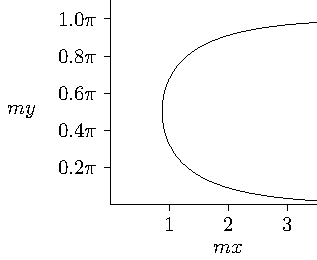
\includegraphics{figLaplaceSimplestBoundaryConditionsExampleA}
\caption{$my=\sin^{-1} \left(\tfrac{1}{\sinh mx}\right)$ کی مساوات۔}
\label{شکل_لاپلاس_سرحدی_شرائط_الف}
\end{figure}
%
\begin{figure}
\centering
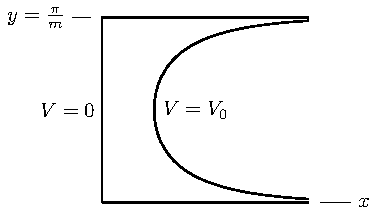
\includegraphics{figLaplaceSimplestBoundaryEquipotentialSurfacesExampleA}
\caption{ہم قوہ سطحیں اور ان پر برقی دباو۔}
\label{شکل_لاپلاس_سرحدی_شرائط_ہم_قوہ_سطحیں_الف}
\end{figure}

ان حقائق کو استعمال کرتے ہوئے موصل ہم قوہ سطحیں شکل \حوالہ{شکل_لاپلاس_سرحدی_شرائط_ہم_قوہ_سطحیں_الف} میں دکھائی گئی ہیں۔یہ سطحیں \عددیء{z} محدد کی سمت میں لامحدود لمبائی رکھتی ہیں اور ان سے پیدا برقی دباو مساوات \حوالہ{مساوات_لاپلاس_اندازہ_ث} دیتا ہے۔

ہم نے لاپلاس مساوات کے حل یعنی مساوات \حوالہ{مساوات_لاپلاس_اندازہ_ث} کو لیتے ہوئے ان ہم قوہ سطحوں کو دریافت کیا جو ایسی برقی دباو پیدا کرے گی۔حقیقت میں عموماً موصل ہم قوہ سطحیں معلوم ہوں گی جن کا پیدا کردہ برقی دباو درکار ہو گا۔آئیں ایسی ایک مثال دیکھیں۔

شکل \حوالہ{شکل_لاپلاس_متعدد_اجزاء_مجموعہ} میں موصل سطحیں اور ان پر برقی دباو دیا گیا ہے۔یہ سطحیں \عددیء{z} سمت میں لامحدود لمبائی رکھتی ہیں۔سطحوں کے  گھیرے خطے میں برقی دباو حاصل کرنا درکار ہے۔

\begin{figure}
\centering
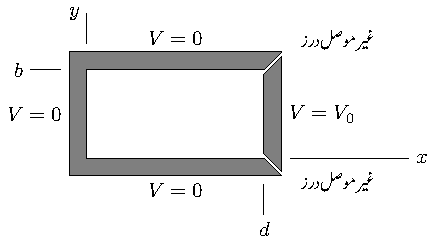
\includegraphics{figLaplaceSimplestBoundaryConditionsExample}
\caption{موصل سطحوں سے گھیرے خطے میں لاپلاس مساوات متعدد اجزاء کے مجموعے سے حاصل ہوتا ہے۔}
\label{شکل_لاپلاس_متعدد_اجزاء_مجموعہ}
\end{figure} 

یہاں سرحدی شرائط کچھ یوں ہیں۔\عددیء{x=0}، \عددیء{y=0} اور \عددیء{y=b} پر برقی دباو صفر ہے جبکہ \عددیء{x=d} پر برقی دباو  \عددیء{V_0} ہے۔دونوں ہم قوہ سطحوں کے مابین انتہائی باریک غیر موصل درز ہیں جن کی بنا پر ان کے برقی دباو مختلف ہو سکتے ہیں۔ان درز کے اثر کو نظرانداز کیا جائے گا۔

موجودہ مسئلے میں بھی برقی دباو صرف \عددیء{x} اور \عددیء{y} کے ساتھ تبدیل ہوتا ہے لہٰذا مساوات \حوالہ{مساوات_لاپلاس_ضربی_حل_الف} ہی اس مسئلے کا لاپلاس مساوات ہے جس کا حل مساوات \حوالہ{مساوات_لاپلاس_اندازہ_ت} ہے۔ہم سرحدی شرائط لاگو کرتے ہوئے مساوات کے مستقل حاصل کرتے ہیں۔مساوات \حوالہ{مساوات_لاپلاس_ضربی_حل_الف} میں \عددیء{x=0} پر برقی دباو صفر پر کرنے سے
\begin{align*}
0&=\left( A \cosh 0+B \sinh 0\right) \left(C \cos m y+D \sin m y \right)\\
0&=A \left(C \cos m y+D \sin m y \right)
\end{align*}
حاصل ہوتا ہے۔ \عددیء{y} کے تمام قیمتوں کے لئے یہ مساوات صرف 
\begin{align*}
A=0
\end{align*}
کی صورت میں درست ہو سکتی ہے لہٰذا پہلا مستقل صفر کے برابر حاصل ہوتا ہے۔\عددیء{y=0} پر صفر برقی دباو پر کرنے سے
\begin{align*}
0&=B \sinh mx  \left(C \cos 0+D \sin 0 \right)\\
0&=BC \sinh mx 
\end{align*}
لکھا جائے گا جو \عددیء{x} کی ہر قیمت کے لئے صرف \عددیء{BC=0} کی صورت میں درست ہو گا۔اب چونکہ \عددیء{A=0} ہے لہٰذا \عددیء{B} صفر نہیں ہو سکتا چونکہ ایسی صورت میں مساوات \حوالہ{مساوات_لاپلاس_ضربی_حل_الف} سے برقی دباو صفر حاصل ہو گا۔یہ جواب ہمیں مطلوب نہیں ہے۔ہم وہ جواب چاہتے ہیں جس سے برقی دباو کے بارے میں علم حاصل ہو۔اس لئے \عددیء{C=0} کے برابر ہے۔اس طرح مساوات \حوالہ{مساوات_لاپلاس_اندازہ_ت}
\begin{align}\label{مساوات_لاپلاس_ڈبہ_مثال}
V&=BD \sinh mx  \sin m y 
\end{align}
صورت اختیار کر لے گی۔اس مساوات میں \عددیء{y=b} پر صفر برقی دباو پر کرتے ہیں۔
 \begin{align*}
0&=BD \sinh mx  \sin m b 
\end{align*}
ہم \عددیء{B} یا \عددیء{D} کو صفر کے برابر نہیں لے سکتے چونکہ ایسی صورت میں \عددیء{V=0} جواب حاصل ہوتا ہے جس میں ہمیں کوئی دلچسپی نہیں۔یہ مساوات \عددیء{x} کی ہر قیمت کے لئے صرف اس صورت درست ہو گی اگر 
\begin{align*}
\sin mb=0
\end{align*}
ہو جس سے
\begin{align*}
mb = n\pi 
\end{align*}
حاصل ہوتا ہے جہاں
\begin{align*}
n=0,1,2,\cdots
\end{align*}
کے برابر ہو سکتا ہے۔اس طرح \عددیء{m=\tfrac{n\pi}{b}} لکھتے ہوئے مساوات \حوالہ{مساوات_لاپلاس_ڈبہ_مثال}
\begin{align}\label{مساوات_لاپلاس_ڈبہ_مثال_تین_شرائط_پورے}
V&=V_1 \sinh \frac{n\pi x}{b}  \sin \frac{n\pi y}{b} 
\end{align}
صورت اختیار کر لے  گا جہاں \عددیء{BD} کو \عددیء{V_1} لکھا گیا ہے۔مساوات \حوالہ{مساوات_لاپلاس_ڈبہ_مثال_تین_شرائط_پورے} تین اطراف کے سطحوں پر صفر برقی دباو کے شرائط پر پورا اترتا حل ہے۔البتہ \عددیء{x=d} پر \عددیء{V_0} برقی دباو کے شرط کو مندرجہ بالا مساوات سے پورا کرنا ممکن نہیں۔ہمیں عموماً بالکل اسی طرز کے مسئلوں سے واسطہ پڑتا ہے جہاں آخری قدم پر معلوم ہوتا ہے کہ ہماری کمر دیوار کے ساتھ لگ گئی ہے جہاں سے ظاہری طور پر نکلنے کا کوئی راستہ نہیں۔گھبرائیں نہیں۔ہمیں درپیش مسئلے کے تمام ممکنہ جوابات کو مساوات \حوالہ{مساوات_لاپلاس_ڈبہ_مثال_تین_شرائط_پورے} کی شکل میں لکھا جا سکتا ہے۔یوں ان تمام جوابات کا مجموعہ بھی قابل قبول حل ہو گا یعنی ہم 
\begin{align}\label{مساوات_لاپلاس_فوریئر_تسلسل_کا_حل}
V=\sum_{n=0}^{\infty} V_{n} \sinh \frac{n\pi x}{b} \sin \frac{n\pi y}{b} \quad \quad (0<y<b,n=0,1,2,\cdots)
\end{align}
بھی لکھ سکتے ہیں جہاں  \عددیء{n} کی ہر قیمت پر منفرد  \عددیء{V_1} کو \عددیء{V_n} سے ظاہر کیا گیا ہے۔ \عددیء{n} اور \عددیء{V_n} کی قیمتیں ایسی رکھی جاتی ہیں کہ  \عددیء{x=d} پر \عددیء{V_0} برقی دباو کے شرط کو پورا کیا جائے۔اس آخری شرط کو مساوات میں پر کرتے ہوئے
\begin{align*}
V_0&=\sum_{n=0}^{\infty} V_{n} \sinh \frac{n\pi d}{b} \sin \frac{n\pi y}{b}
\end{align*}
یعنی
\begin{align}\label{مساوات_لاپلاس_فوریئر_تسلسل_حل}
V_0=\sum_{n=0}^{\infty} c_n\sin \frac{n\pi y}{b}
\end{align}
ملتا ہے جہاں 
\begin{align*}
c_n=V_n \sinh \frac{n\pi d}{b}
\end{align*}
لکھا گیا ہے۔

مساوات \حوالہ{مساوات_لاپلاس_فوریئر_تسلسل_حل} \اصطلاح{فوریئر تسلسل}\فرہنگ{فوریئر تسلسل}\حاشیہب{Fourier series}\فرہنگ{Fourier series} ہے جس کے مستقل با آسانی حاصل کئے جا سکتے ہیں۔چونکہ ہمیں \عددیء{0<y<b} کے خطے سے غرض ہے لہٰذا اس خطے کے باہر ہمیں برقی دباو سے کوئی غرض نہیں۔ایسی صورت میں ہم فوریئر تسلسل کے طاق یا جفت جوابات حاصل کر سکتے ہیں۔طاق جوابات اس صورت حاصل ہوں گے اگر ہم \عددیء{0<y<b} کو آدھا میعاد تصور کرتے ہوئے بقایا آدھے میعاد \عددیء{b<y<2b} پر برقی دباو کو \عددیء{-V_0} تصور کریں یعنی  
\begin{align*}
V&=+V_0 \quad \quad (0<y<b)\\
V&=-V_0 \quad \quad (b<y<2b)
\end{align*}
اسی صورت میں فوریئر تسلسل کے مستقل
\begin{align*}
c_n=\frac{1}{b}\left[\int_{0}^{b} V_0 \sin \frac{n\pi y}{b} \dif y +\int_{b}^{2b} (-V_0) \sin \frac{n\pi y}{b} \dif y \right]
\end{align*}
سے
\begin{align*}
c_n&=\frac{4V_0}{n\pi} \quad \quad (n=1,3,5,\cdots)\\
c_n&=0 \quad \quad (n=2,4,6,\cdots)
\end{align*}
حاصل ہوتے ہیں۔اب چونکہ \عددیء{c_n=V_n\sinh \tfrac{n\pi d}{b}} کے برابر ہے لہٰذا
\begin{align*}
V_n=\frac{4V_0}{n \pi \sinh (\tfrac{n \pi d}{b})}  \quad \quad (n=1,3,5,\cdots)
\end{align*}
ہو گا اور یوں مساوات \حوالہ{مساوات_لاپلاس_فوریئر_تسلسل_کا_حل} کو
\begin{align}\label{مساوات_لاپلاس_طاقتی_تسلسل_مساوات}
V=\frac{4V_0}{\pi} \sum_{n=1,\text{طاق}}^{\infty} \frac{1}{n} \frac{\sinh \frac{n\pi x}{b}}{\sinh \tfrac{n\pi d}{b}} \sin \frac{n\pi y}{b}
\end{align}
لکھا جا سکتا ہے۔اس مساوات سے مختلف نقطوں پر برقی دباو \عددیء{V(x,y)} حاصل کرتے ہوئے  ان میں برابر برقی دباو رکھنے والے نقطوں سے گزرتی سطح ہم قوہ سطح ہو گی۔

%======================
\ابتدا{مثال}\شناخت{مثال_لاپلاس_طاقتی_تسلسل_ایک_چادر_پر_دباو}
شکل \حوالہ{شکل_لاپلاس_متعدد_اجزاء_مجموعہ} میں \عددیء{d=b} اور \عددیء{V_0=\SI{90}{\volt}} ہونے کی صورت میں ڈبے کے عین وسط میں برقی دباو حاصل کریں۔

حل:ڈبے کا وسط \عددیء{(\tfrac{b}{2},\tfrac{b}{2})} ہے۔مساوات \حوالہ{مساوات_لاپلاس_طاقتی_تسلسل_مساوات} کے پہلے چند اجزاء لیتے ہوئے
\begin{align*}
V&=\frac{4\times 90}{\pi} \left( \frac{\sinh \frac{\pi}{2}}{\sinh \pi} \sin \frac{\pi}{2}+\frac{1}{3}  \frac{\sinh \frac{3\pi}{2}}{\sinh 3\pi} \sin \frac{3\pi}{2}+\frac{1}{5}  \frac{\sinh \frac{5\pi}{2}}{\sinh 5\pi} \sin \frac{5\pi}{2}\right)\\
&=\frac{4\times 90}{\pi} \left(0.199268-0.0029941887+0.0000776406 \right)\\
&=\SI{22.5}{\volt}
\end{align*}
حاصل ہوتا ہے۔
\انتہا{مثال}
%=======================
\حصہ{اعدادی دہرانے کا طریقہ}
لاپلاس مساوات حل کرنے کے کئی تراکیب ہم دیکھ چکے۔کمپیوٹر کی مدد سے \اصطلاح{اعدادی دہرانے}\فرہنگ{اعدادی دہرانا}\فرہنگ{دہرانا!اعدادی}\حاشیہب{numerical iteration}\فرہنگ{numerical iteration}\فرہنگ{iteration!numerical} کے طریقے سے مساوات حل کئے جاتے ہیں۔آئیں لاپلاس مساوات اسی ترکیب سے حل کریں۔
  
\begin{figure}
\centering
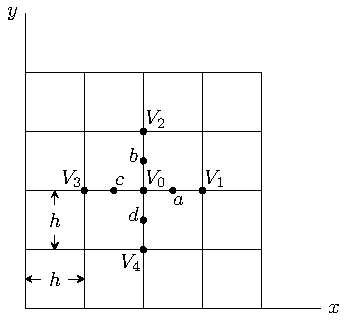
\includegraphics{figLaplaceIterationProcessDefined}
\caption{لاپلاس مساوات کے تحت کسی بھی نقطے پر برقی دباو قریبی نقطوں کے برقی دباو کا اوسط ہوتا ہے۔}
\label{شکل_لاپلاس_برقی_دباو_اوسط_قیمت_ہی_ہے}
\end{figure}
تصور کرتے ہیں کہ کسی خطے میں برقی میدان صرف \عددیء{x} اور \عددیء{y} کے ساتھ تبدیل ہوتا ہے۔شکل \حوالہ{شکل_لاپلاس_برقی_دباو_اوسط_قیمت_ہی_ہے} میں ایسی سطح دکھائی گئی ہے جسے \عددیء{h} چوڑائی اور اتنے ہی لمبائی کے مربع کے ٹکڑوں میں تقسیم کیا گیا ہے۔اس میدان میں آپس میں قریبی پانچ نقطوں پر برقی دباو \عددیء{V_0}، \عددیء{V_1}، \عددیء{V_2}، \عددیء{V_3} اور  \عددیء{V_4} ہیں۔اگر یہ خطہ ہر جانب یکساں خاصیت رکھتا ہو اور یہ بار سے پاک ہو تب \عددیء{\nabla \cdot \kvec{D}=0} اور \عددیء{\nabla \cdot \kvec{E}=0} ہوں گے جس سے دو محدد میں
\begin{align*}
\frac{\partial E_x}{\partial x}+\frac{\partial E_y}{\partial y}=0
\end{align*}
لکھا جا سکتا ہے۔اب \عددیء{E_x=-\tfrac{\partial V}{\partial x}} اور \عددیء{E_y=-\tfrac{\partial V}{\partial y}} ہونے کی وجہ سے مندرجہ بالا مساوات 
\begin{align*}
\frac{\partial^2 V}{\partial x}+\frac{\partial^2 V}{\partial y^2}=0
\end{align*}
صورت اختیار کر لیتی ہے جو لاپلاس مساوات ہے۔شکل \حوالہ{شکل_لاپلاس_برقی_دباو_اوسط_قیمت_ہی_ہے} میں نقطہ \عددیء{a} اور نقطہ \عددیء{c} پر \عددیء{\tfrac{\partial V}{\partial x}} اور \عددیء{\tfrac{\partial V}{\partial y}} کی قیمتیں تقریباً
\begin{align*}
\eval{\frac{\partial V}{\partial x}}_a&\overset{.}{=}\frac{V_1-V_0}{h}\\
\eval{\frac{\partial V}{\partial x}}_c&\overset{.}{=}\frac{V_0-V_3}{h}
\end{align*}
ہوں گیں۔یوں ہم
\begin{align*}
\eval{\frac{\partial^2 V}{\partial x^2}}_0\overset{.}{=}\frac{\eval{\frac{\partial V}{\partial x}}_a-\eval{\frac{\partial V}{\partial x}}_c}{h}
\overset{.}{=}\frac{V_1-V_0-V_0+V_3}{h^2}
\end{align*}
لکھ سکتے ہیں۔بالکل اسی طرح ہم
\begin{align*}
\eval{\frac{\partial^2 V}{\partial y^2}}_0\overset{.}{=}\frac{\eval{\frac{\partial V}{\partial y}}_b-\eval{\frac{\partial V}{\partial y}}_d}{h}
\overset{.}{=}\frac{V_2-V_0-V_0+V_4}{h^2}
\end{align*}
بھی لکھ سکتے ہیں۔ان دو جوابات کو لاپلاس مساوات میں پر کرنے
\begin{align*}
\frac{\partial^2 V}{\partial x^2}+\frac{\partial^2 V}{\partial y^2}\overset{.}{=}\frac{V_1+V_2+V_3+V_4-4V_0}{h^2}=0
\end{align*}
سے
\begin{align}\label{مساوات_لاپلاس_عددی_دہرانے_کا_طریقہ}
V_0\overset{.}{=}\frac{V_1+V_2+V_3+V_4}{4}
\end{align}
حاصل ہوتا ہے۔\عددیء{h} لمبائی جتنی کم ہو مندرجہ بالا مساوات اتنی زیادہ درست ہو گی۔\عددیء{h} کی لمبائی انتہائی چھوٹی کرنے سے مندرجہ بالا مساوات بالکل صحیح ہو گی۔یہ مساوات  کہتی ہے کہ کسی بھی نقطے پر برقی دباو اس نقطے کے گرد چار نقطوں کے برقی دباو کا اوسط ہوتا ہے۔

اعدادی دہرانے کے طریقے میں تمام خطے کو شکل \حوالہ{شکل_لاپلاس_برقی_دباو_اوسط_قیمت_ہی_ہے} کی طرز پر مربعوں میں تقسیم کرتے ہوئے مربع کے ہر کونے پر  مساوات \حوالہ{مساوات_لاپلاس_عددی_دہرانے_کا_طریقہ} کی مدد سے برقی دباو حاصل کیا جاتا ہے۔تمام خطے پر بار بار اسی طریقے سے برقی دباو حاصل کیا جاتا ہے حتٰی کہ کسی بھی نقطے پر متواتر جوابات میں  تبدیلی نہ پائی جائے۔اس طریقے کو مثال سے بہتر سمجھا جا سکتا ہے۔

\begin{figure}
\centering
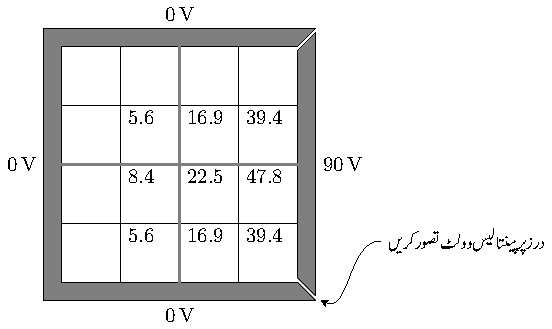
\includegraphics{figLaplaceIterationExample}
\caption{رقبہ عمودی تراش کو خانوں میں تقسیم کرتے ہوئے، ہر کونے پر گرد کے چار نقطوں کے اوسط برابر برقی دباو ہو گا۔}
\label{شکل_لاپلاس_دہرانے_کا_طریقہ}
\end{figure}

شکل \حوالہ{شکل_لاپلاس_دہرانے_کا_طریقہ} میں مربع شکل کے لامحدود لمبائی کے ڈبے کا عمودی تراش دکھایا گیا ہے۔اس کے چار اطراف صفر برقی دباو پر ہیں جبکہ نہایت باریک غیر موصل فاصلے پر چوتھی طرف نوے وولٹ پر ہے۔اس ڈبے کو یوں خانوں میں تقسیم کیا گیا ہے کہ یا تو انہیں سولہ چھوٹے خانے تصور کیا جا سکتا ہے اور یا چار درمیانے جسامت کے خانے۔اس کے علاوہ پورے ڈبے کو ایک ہی بڑا خانہ بھی تصور کیا جا سکتا ہے۔آئیں ان خانوں کے کونوں پر مساوات \حوالہ{مساوات_لاپلاس_عددی_دہرانے_کا_طریقہ} کی مدد سے برقی دباو حاصل کریں۔

اگرچہ کمپیوٹر پر ایسے مسائل حل کرتے ہوئے تمام کونوں پر ابتدائی برقی دباو صفر تصور کرتے ہوئے آگے بڑھا جاتا ہے۔قلم و کاغذ استعمال کرتے ہوئے ذرا سوچ کر چلنا بہتر ثابت ہوتا ہے۔ہم پورے مربع شکل کو ایک ہی بڑا خانہ تصور کرتے ہوئے اس کے عین وسط میں برقی دباو حاصل کرتے ہیں۔ایسا کرنے کی خاطر ہم بڑے خانے کے چار کونوں کو قریبی نقطے چنتے ہیں۔یوں بڑے خانے کے چار کونوں کی برقی دباو زیر استعمال آئے گی۔اب دو کونوں پر صفر برقی دباو ہے جبکہ دو کونے غیر موصل درز پر مشتمل ہیں۔درز کے ایک جانب صفر جبکہ اس کی دوسری جانب نوے وولٹ ہیں، لہٰذا درز میں ان دو قیمتوں کا اوسط یعنی پینتالیس وولٹ برقی دباو تصور کیا جا سکتا ہے۔ اس طرح بڑے خانے کے وسط میں
\begin{align*}
V=\frac{45+45+0+0}{4}=\SI{22.5}{\volt}
\end{align*}
حاصل ہوتا ہے۔شکل \حوالہ{شکل_لاپلاس_دہرانے_کا_طریقہ} میں یہ قیمت دکھائی گئی ہے۔

آئیں اب چار درمیانے جسامت کے خانوں کے کونوں پر برقی دباو حاصل کریں۔یہاں بھی ہم ان خانوں کے کونوں کو چار قریبی نقطے چنتے ہیں۔اوپر دائیں بڑے خانے کے وسط میں برقی دباو حاصل کرنے کی خاطر اس خانے کے چار کونوں کے برقی دباو زیر استعمال لائے جائیں گے۔یوں درز پر پینتالیس وولٹ تصور کرتے ہوئے
\begin{align*}
V=\frac{90+45+0+22.5}{4}=\SI{39.4}{\volt}
\end{align*}
حاصل ہوتے ہیں۔اسی طرح دائیں نچلے بڑے خانے کے وسط میں بھی
\begin{align*}
V=\frac{90+45+0+22.5}{4}=\SI{39.4}{\volt}
\end{align*}
حاصل ہوتا ہے۔ہم اس قیمت کو بغیر حل کئے شکل کو دیکھ کر ہی لکھ سکتے تھے چونکہ شکل کا اوپر والا آدھا حصہ اور اس کا نچلا آدھا حصہ بالکل یکساں ہیں لہٰذا ان دونوں حصوں میں بالکل یکساں برقی دباو ہو گا۔اس حقیقت کو یہاں سے استعمال کرنا شروع کرتے ہیں۔اوپر اور نیچے بائیں بڑے خانے بالکل یکساں ہیں لہٰذا دونوں کے وسط میں
\begin{align*}
V=\frac{22.5+0+0+0}{4}=\SI{5.6}{\volt}
\end{align*}
حاصل ہوتے ہیں۔بقایا کونوں پر برقی دباو حاصل کرتے ہوئے نقطے کے بائیں، دائیں، اوپر اور نیچے نقطوں کو قریبی نقطے چنتے ہیں۔یوں
\begin{align*}
\frac{90+39.4+22.5+39.4}{4}&=\SI{47.8}{\volt}\\
\frac{39.4+0+5.6+22.5}{4}&=\SI{16.9}{\volt}\\
\frac{22.5+5.6+0+5.6}{4}&=\SI{8.4}{\volt}
\end{align*}
حاصل ہوتے ہیں۔شکل \حوالہ{شکل_لاپلاس_دہرانے_کا_طریقہ} میں یہ تمام قیمت دکھائی گئی ہے۔

\begin{figure}
\centering
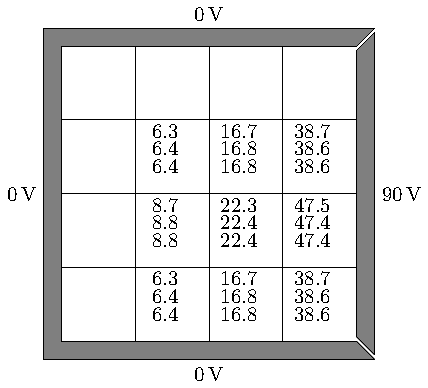
\includegraphics{figLaplaceIterationExampleWorkedTillStableAnswers}
\caption{چار مرتبہ دہرانے کے بعد جوابات تبدیل ہونا بند ہو جاتے ہیں۔یہی اصل جواب ہیں۔}
\label{شکل_لاپلاس_دہرانے_کے_اٹل_جواب}
\end{figure}

آئیں شکل میں اوپر سے نیچے چلتے ہوئے پہلے دائیں، پھر درمیانے اور آخر میں بائیں قطار  کے تمام کونوں پر برقی دباو حاصل کریں۔ہم یہی سلسلہ بار بار دہرائیں گے حتٰی کہ کسی بھی کونے پر متواتر حاصل کردہ جوابات تبدیل ہونا بند کر دیں۔ہر کونے پر برقی دباو مساوات \حوالہ{مساوات_لاپلاس_عددی_دہرانے_کا_طریقہ} کے استعمال سے حاصل کیا جائے گا جہاں کونے کے اوپر، نیچے، دائیں اور بائیں نقطوں کے برقی دباو کو استعمال کیا جائے گا۔یاد رہے کہ موصل سطحوں پر برقی دباو ہمیں پہلے  سے ہی معلوم ہے لہٰذا ان پر برقی دباو حاصل کرنے کی کوشش نہیں کی جائے گی۔

اس طرح دائیں قطار کے اوپر جانب \عددیء{\SI{39.4}{\volt}} کی نئی قیمت
\begin{align*}
\frac{90+0+16.9+47.8}{4}=\SI{38.7}{\volt}
\end{align*}
ہو جائے گی۔اوپر اور نچلے آدھے حصوں کی مشابہت سے ہم قطار کی نچلی قیمت بھی یہی لکھتے ہیں۔شکل \حوالہ{شکل_لاپلاس_دہرانے_کے_اٹل_جواب} میں یہ قیمتیں دکھائی گئی ہیں۔مساوات  \حوالہ{مساوات_لاپلاس_عددی_دہرانے_کا_طریقہ} میں نئی سے نئی قیمتیں استعمال کی جاتی ہیں۔یوں \عددیء{\SI{47.8}{\volt}} کی نئی قیمت
\begin{align*}
\frac{90+38.7+22.5+38.7}{4}=\SI{47.5}{\volt}
\end{align*}
ہو گی۔

درمیانی قطار پر آتے ہیں۔یہاں اوپر \عددیء{\SI{16.9}{\volt}} کی نئی قیمت
\begin{align*}
\frac{38.7+0+5.6+22.5}{4}=\SI{16.7}{\volt}
\end{align*}
ہو گی جو قطار کے  نچلے کونے کی بھی قیمت ہے۔اس قطار کے درمیانے نقطے کی نئی قیمت
\begin{align*}
\frac{47.5+16.7+8.4+16.7}{4}=\SI{22.3}{\volt}
\end{align*}
ہو گی۔

اسی طرح بائیں قطار  کی نئی قیمتیں بھی حاصل کی جاتی ہیں۔ان تمام کو شکل \حوالہ{شکل_لاپلاس_دہرانے_کے_اٹل_جواب} میں دکھایا گیا ہے۔یہی سلسلہ دوبارہ دہرانے سے مزید نئے اور بہتر جوابات حاصل ہوں گے جنہیں گزشتہ جوابات کے نیچے لکھا گیا ہے۔شکل میں اس طرح تین مرتبہ دہرانے سے حاصل کئے گئے جوابات دکھائے گئے ہیں۔آپ دیکھ سکتے ہیں کہ کسی بھی نقطے کے آخری دو حاصل کردہ جوابات میں کوئی تبدیلی نہیں پائی جاتی۔اسی لئے ان آخری جوابات کو حتمی جوابات تسلیم کیا جاتا ہے۔

یہاں ڈبے کے عین وسط میں برقی دباو \عددیء{\SI{22.4}{\volt}} حاصل ہوا ہے۔مثال \حوالہ{مثال_لاپلاس_طاقتی_تسلسل_ایک_چادر_پر_دباو} میں ڈبے کے وسط پر برقی دباو طاقتی سلسلے کی مدد سے \عددیء{\SI{22.5}{\volt}} حاصل ہوئی تھی جو تقریباً اتنی ہی قیمت ہے۔یاد رہے کہ یہاں ہم نے اشاریہ کے بعد صرف ایک ہندسہ رکھتے ہوئے برقی دباو حاصل کئے۔اسی وجہ سے دونوں جوابات میں معمولی فرق ہے۔ 

اگر ہم سوچ سے کام نہ لیتے ہوئے سیدھ و سیدھ مساوات \حوالہ{مساوات_لاپلاس_عددی_دہرانے_کا_طریقہ} میں شروع سے دائیں، بائیں، اوپر اور نیچے نقطوں کی قیمتیں استعمال کرتے، تب ہمیں قطعی جوابات دس مرتبہ دہرانے کے بعد حاصل ہوتے۔اگرچہ قلم و کاغذ استعمال کرتے ہوئے آپ ضرور سوچ سمجھ سے ہی کام لیں گے البتہ کمپیوٹر استعمال کرتے ہوئے ایسا کرنے کی ضرورت پیش نہیں آتی۔کمپیوٹر کے لئے کیا ایک مرتبہ اور کیا دس ہزار مرتبہ۔

اس مثال میں ہم نے بہت کم نقطوں پر برقی دباو حاصل کی تا کہ دہرانے کا طریقہ با آسانی سمجھا جا سکے۔کمپیوٹر استعمال کرتے ہوئے آپ زیادہ سے زیادہ نقطے چن سکتے ہیں۔بہتر سے بہتر نتائج، زیادہ سے زیادہ نقطے چننے سے حاصل ہوتا ہے نا کہ کم نقطوں پر زیادہ ہندسوں پر مبنی جوابات سے۔دہرانے کا طریقہ اس مرتبہ تک دہرایا جاتا ہے جب تک کسی بھی نقطے پر دو متواتر حاصل کردہ جوابات میں فرق اتنا کم ہو کہ اسے رد کرنا ممکن ہو۔یوں ایک مائیکرو وولٹ تک درست جوابات حاصل کرنے کی خاطر اس وقت تک دہرائی کی جائے گی جب تک کسی بھی نقطے پر دو متواتر جوابات میں فرق ایک مائیکرو وولٹ سے کم نہ ہو جائے۔    
%===============

\newpage

\حصہء{سوالات}
%======================
\ابتدا{سوال}
برقی دباو \عددی{V=0.002x^2yz^3 \, \si{\volt}} ہے۔نقطہ \عددی{N(2,-3,-4)} پر \عددی{V}، \عددی{\kvec{E}} اور \عددی{\abs{\rho_h}} حاصل کریں۔نقطہ \عددی{N} پر ہم قوہ سطح اور سمت بہاو خط کی مساوات حاصل کریں۔کیا برقی دباو لاپلاس کی مساوات پر پورا اترتا ہے؟

جوابات: \عددی{\SI{1.536}{\volt}}، \عددی{\kvec{E}=-1.536\ax+0.512\ay+1.152\az \, \si{\volt\per\meter}}،
 \عددی{\abs{\rho_h}=\SI{1.344}{\coulomb\per\meter\squared}}، \عددی{x^2yz^3-768=0}؛ سمت بہاو خط ان مساوات سے ظاہر ہو گی: \عددی{2y^2-x^2=14} اور \عددی{2z^2-3x^2=6}؛ چونکہ حاصل کردہ حجمی کثافت بار صفر کے برابر نہیں ہے لہٰذا لاپلاس کی مساوات پر برقی دباو پورا نہیں اترتا۔
\انتہا{سوال}
%========================
\ابتدا{سوال}
دباو کا میدان \عددی{V=xy^2z-kxz^3} لاپلاس مساوات پر پورا اترتا ہے۔مستقل \عددی{k} کی قیمت حاصل کرتے ہوئے نقطہ \عددی{N(5,2,4)} پر \عددی{\kvec{E}} کی سمت میں اکائی سمتیہ دریافت کریں۔

جوابات:\عددی{k=\tfrac{1}{3}}، \عددی{0.053\ax-0.799\ay+0.599\az}
\انتہا{سوال}
%=========================
\ابتدا{سوال}
خلاء میں نقطہ \عددی{N(2,-3,1)} پر میدان \عددی{V=x+y^2(z^3-x^2)} اور \عددی{V=3x^2+y^2-4z^2} میں \عددی{\rho_h} حاصل کریں۔

جوابات:\عددی{\SI{-0.265}{\nano\coulomb\per\meter^3}}، \عددی{\SI{0}{\coulomb\per\meter^3}}
\انتہا{سوال}
%========================
\ابتدا{سوال}
محدد کے مبدا \عددی{(0,0,0)} پر \عددی{V=3x^3+y^4+2z}  اور \عددی{V=e^{2x}\sin 2y} کے لاپلاس کی قیمت حاصل کریں۔ کیا یہ تفاعل لاپلاس مساوات پر پورا اترتے ہیں؟
جوابات: \عددی{0}، \عددی{0}، نہیں، جی ہاں
\انتہا{سوال}
%========================
\ابتدا{سوال}
میدان \عددی{V=5\rho^2 \sin 2\phi} کا لاپلاس حاصل کریں۔

جواب: \عددی{\nabla^2 V=0}
\انتہا{سوال}
%========================
\ابتدا{سوال}
ثابت کریں کہ \عددی{V=\rho V_0 \cos \phi} لاپلاس مساوات پر پورا اترتا ہے۔اسی برقی دباو کو کارتیسی محدد میں لکھتے ہوئے \عددی{V=0} اور \عددی{V=V_0} سطحیں دریافت کریں۔

جوابات:\عددی{V=V_0 x}، \عددی{x=0}، \عددی{x=1}
\انتہا{سوال}
%======================
\ابتدا{سوال}
متوازی چادر برق گیر (کپیسٹر)  میں \عددی{{V=10x+15y-30z+55}} ہے۔ چادر کا رقبہ \عددی{\SI{100}{\centi\meter\squared}} جبکہ ان کے درمیان فاصلہ \عددی{\SI{0.5}{\milli\meter}} ہے۔برق گیر (کپیسٹر)  پر برقی دباو کی قیمت حاصل کریں۔اس کی کپیسٹنس بھی حاصل کریں۔

جوابات:\عددی{\SI{17.5}{\milli\volt}}، \عددی{\SI{177}{\pico\farad}}
\انتہا{سوال}
%====================
\ابتدا{سوال}
نلکی محدد میں میدان \عددی{V(\rho,\phi,z)=55\phi+72 \, \si{\volt}} دیا گیا ہے۔نقطہ \عددی{N(2.2,62^{\circ},3)} پر \عددی{V}، \عددی{\kvec{E}} اور کثافت توانائی حاصل کریں۔خطہ \عددی{\rho_1} تا \عددی{\rho_2}، \عددی{\phi_1} تا \عددی{\phi_2}،  \عددی{z_1} تا \عددی{z_2} میں کل توانائی حاصل کریں۔

جوابات: \عددی{\SI{132}{\volt}}، \عددی{-25\aphi \, \si{\volt\per\meter}}، \عددی{\SI{2.77}{\nano\joule\per\meter^3}}،
 \عددی{13.4(\phi_2-\phi_1)(z_2-z_1)\ln \tfrac{\rho_2}{\rho_1} \, \si{\nano\joule}}
\انتہا{سوال}
%=====================
\ابتدا{سوال}
متوازی چادر برق گیر (کپیسٹر)  کے چادروں کے درمیان فاصلہ \عددی{d} اور برقی مستقل \عددی{\epsilon} ہے۔دونوں چادر صفر وولٹ پر ہیں جبکہ ان کے درمیان خطے  میں حجمی کثافت بار \عددی{\rho_h} پائی جاتی ہے۔پوئسن  مساوات حل کرتے ہوئے چادروں کے درمیان برقی دباو اور \عددی{\kvec{E}} حاصل کریں۔

جوابات:\عددی{V(z)=\tfrac{\rho_0 z}{2 \epsilon}(d-z) \, \si{\volt}}، \عددی{\kvec{E}=\tfrac{\rho_0}{2\epsilon}(2z-d)\az \, \si{\volt\per\meter}} 
\انتہا{سوال}
%==================
\ابتدا{سوال}
نلکی محدد استعمال کرتے ہوئے خلاء میں برقی دباو کی مساوات \عددی{V=\tfrac{\sin 2 \phi}{\rho}} دی گئی ہے۔ نقطہ \عددی{(0.4,45^{\circ},2)} پر حجمی کثافت بار \عددی{\rho_h} حاصل کریں۔نقطہ \عددی{(2.5,75^{\circ},3)} پر موصل سطح موجود ہے۔اس پر سطحی کثافت بار \عددی{\rho_S} حاصل کریں۔

جوابات: \عددی{\SI{415}{\pico\coulomb\per\meter^3}}، \عددی{\SI{\mp 2.55}{\pico\coulomb\per\meter\squared}}؛چونکہ یہ نہیں بتلایا گیا کہ میدان موصل کے کس جانب ہے لہٰذا یہ نہیں بتلایا جا سکتا کہ کثافت مثبت یا منفی ہے۔
\انتہا{سوال}
%=====================
\ابتدا{سوال}
رداس \عددی{a} کے دو عدد دائری چادر سے متوازی چادر برق گیر (کپیسٹر)  بنایا جاتا ہے۔یہ چادر \عددی{z=0} اور \عددی{z=d} پر پائے جاتے ہیں جبکہ \عددی{z} محدد ان کے محور سے گزرتی ہے۔نچلی چادر صفر وولٹ جبکہ بالائی چادر \عددی{V_0} وولٹ پر ہے۔برق گیر (کپیسٹر)  میں بھرے گئی ذو برق کا برقی مستقل \عددی{\epsilon(\rho)=\epsilon-0(1+\tfrac{\rho}{a})} ہے جو رداسی سمت میں تبدیل ہوتا ہے۔برق گیر (کپیسٹر)  میں \عددی{V} اور \عددی{\kvec{E}} حاصل کریں۔بالائی چادر پر برقی بار حاصل کرتے ہوئے کپیسٹنس حاصل کریں۔چادر کے کناروں پر میدان کے پھولنے\فرہنگ{پھولنا}\حاشیہب{fringing}\فرہنگ{fringing} کو نظر انداز کریں۔

جوابات:چونکہ  \عددی{\kvec{E}} محدد \عددی{z} کی سمت میں ہے جبکہ \عددی{\epsilon} محدد \عددی{\rho} کی سمت میں تبدیل ہوتا ہے لہٰذا لاپلاس اور پوئسن کے مساوات قابل استعمال ہیں۔یوں \عددی{{V(z)=\tfrac{V_0 z }{d}}}،  \عددی{\kvec{E}=-\tfrac{V_0}{d}}، \عددی{\rho_S=\epsilon_0(1+\tfrac{\rho}{d})\tfrac{V_0}{d}}، \عددی{Q=\tfrac{5\pi a^2 \epsilon_0 V_0}{3d}} اور \عددی{C=\tfrac{5\pi a^2 \epsilon_0}{3d}} ہیں۔
\انتہا{سوال}
%======================
\ابتدا{سوال}
صفحہ \حوالہصفحہ{مساوات_لاپلاس_عمومی_لاپلاسی} پر مساوات \حوالہ{مساوات_لاپلاس_عمومی_لاپلاسی} عمومی محدد میں لاپلاسی دیتا ہے۔اس مساوات کو حاصل کریں۔
\انتہا{سوال}
%=============
\ابتدا{سوال}
مثال \حوالہ{مثال_لاپلاس_رداسی_چادروں_کا_کپیسٹر} کو حتمی نتیجے تک پہنچاتے ہوئے اس  کا کپیسٹنس حاصل کریں۔
\انتہا{سوال}
%====================
\ابتدا{سوال}
مثال \حوالہ{مثال_لاپلاس_کروی_رداسی_لاپلاسی} میں دیے مساوات \حوالہ{مساوات_لاپلاس_کروی_رداسی_لاپلاسی_دباو} اور مساوات \حوالہ{مساوات_لاپلاس_کروی_رداسی_لاپلاسی_کپیسٹنس} حاصل کریں۔
\انتہا{سوال}
%=====================
\ابتدا{سوال}
مساوات \حوالہ{مساوات_لاپلاس_مخروطی_حل} کے تکمل کو حل کریں۔
\انتہا{سوال}
%==================
\ابتدا{سوال}
مساوات \حوالہ{مساوات_لاپلاس_مخروطی_حل_ب} حاصل کریں۔
\انتہا{سوال}
%========================
\ابتدا{سوال}
مساوات \حوالہ{مساوات_لاپلاس_مخروطی_کپیسٹنس} حل کریں۔
\انتہا{سوال}
%==========================
\ابتدا{سوال}
مساوات \حوالہ{مساوات_لاپلاس_تفرقی_اجزاء_مستقل_کے_برابر_ب} کے دوسرے جزو کا حل طاقتی سلسلے کے طریقے سے حاصل کریں۔ثابت کریں کہ اس حل کو مساوات \حوالہ{مساوات_لاپلاس_طاقتی_حل_دو_درجی_کارتیسی} کی شکل میں لکھا جا سکتا ہے۔
\انتہا{سوال}
%===============
\ابتدا{سوال}
دہرانے کے طریقے میں اشاریہ کے نشان کے بعد دو ہندسوں تک درستگی استعمال کرتے ہوئے شکل \حوالہ{شکل_لاپلاس_دہرانے_کا_طریقہ} میں دئے تمام نقطوں پر برقی دباو چار مرتبہ دہرانے سے حاصل کریں۔ڈبے کے وسط میں برقی دباو کیا حاصل ہوتی ہے۔

جواب: \عددیء{\SI{22.49}{\volt}}
\انتہا{سوال}
